\documentclass[aspectratio=169,10pt]{beamer}

\usetheme{Madrid}
\usecolortheme{seahorse}
\usefonttheme{professionalfonts}

\usepackage{amsmath,amssymb,amsthm}
\usepackage{mathtools}
\usepackage{listings}
\usepackage{xcolor}
\usepackage{booktabs}
\usepackage{graphicx}
\usepackage{algorithm}
\usepackage{algpseudocode}
\usepackage{multirow}

\graphicspath{{figures/}}

%% Python style
\lstdefinestyle{python}{
  language=Python,
  basicstyle=\ttfamily\scriptsize,
  keywordstyle=\color{blue!80!black}\bfseries,
  stringstyle=\color{orange!80!black},
  commentstyle=\color{green!50!black}\itshape,
  numberstyle=\tiny\color{gray},
  numbers=left, stepnumber=1,
  frame=single, breaklines=true,
  showstringspaces=false, tabsize=4,
  backgroundcolor=\color{gray!7},
}

\title[MC Theory -- Ch.5]{Lectures on Monte Carlo Theory}
\subtitle{Chapter 5: Variance Reduction Techniques}
\author{Based on Lorek \& Rolski}
\date{}

\setbeamertemplate{navigation symbols}{}
\setbeamertemplate{footline}[frame number]

\begin{document}

% ------------------------------------------------------------------ title
\begin{frame}
  \titlepage
\end{frame}

% ------------------------------------------------------------------ TOC
\begin{frame}{Chapter 5 Outline}
  \tableofcontents
\end{frame}

% ==============================================================================
\section{5.1 Survey of Variance Reduction Methods}
% ==============================================================================

\begin{frame}[allowframebreaks]{Motivation: Why Reduce Variance?}

The crude Monte Carlo (CMC) estimator computes $I = \mathbb{E}[Y]$ by averaging
$R$ independent copies of $Y$:
\[
  \hat{Y}_R^{\mathrm{CMC}} = \frac{1}{R}\sum_{j=1}^{R} Y_j,
\]
where $Y_1, \ldots, Y_R$ are i.i.d.\ replications of $Y$, $R$ (capital R) is the
number of replications, and $\hat{Y}_R^{\mathrm{CMC}}$ (Y-hat, CMC) is the
estimate of $I = \mathbb{E}[Y]$ (expected value, i.e., average, of $Y$).

The variance of this estimator is $\mathrm{Var}(\hat{Y}_R^{\mathrm{CMC}}) =
\mathrm{Var}(Y)/R$, meaning the variance (spread of estimates around the true
value) shrinks as we use more replications, but at a slow rate.

\begin{alertblock}{The Fundamental Problem: Diminishing Returns}
The half-width of a 95\% confidence interval is $b \approx 1.96\,\sigma_Y/\sqrt{R}$,
where $\sigma_Y$ (sigma, meaning standard deviation of $Y$) is the square root of
$\mathrm{Var}(Y)$.
To halve the error $b$, we need \emph{four times} as many samples.
Reducing $\mathrm{Var}(Y)$ by a factor $k$ is equivalent to running $k$ times more
simulations -- without the extra cost.
\end{alertblock}

\framebreak

The goal of variance reduction is to construct a new estimator
$\hat{Y}_R^{\mathrm{new}}$ of $I$ satisfying two requirements:
\begin{enumerate}
  \item \textbf{Consistency:} $\hat{Y}_R^{\mathrm{new}} \to I$ with probability 1
        as $R \to \infty$ (it converges to the right answer).
  \item \textbf{Central Limit Theorem (CLT):}
        $\sqrt{R}(\hat{Y}_R^{\mathrm{new}} - I) \xrightarrow{\mathcal{D}} \mathcal{N}(0,\,(\varsigma^{\mathrm{new}})^2)$
        where $\varsigma$ (varsigma, a variant of sigma) is the asymptotic standard deviation,
        and $\mathcal{D}$ (D with arrow) means ``converges in distribution.''
\end{enumerate}

The quantity $(\varsigma^{\mathrm{new}})^2$ is called the
\emph{time-average variance constant} (TAVC) or \emph{asymptotic variance},
defined as $(\varsigma^{\mathrm{new}})^2 = \lim_{R\to\infty} R\,\mathrm{Var}(\hat{Y}_R^{\mathrm{new}})$.
A smaller TAVC means a tighter confidence interval for the same computational budget.

\begin{block}{Methods Covered in This Chapter}
  \begin{enumerate}
    \item Stratified sampling (str)
    \item Antithetic variates (anti)
    \item Common random numbers (CRN)
    \item Ratios of expectations (RoE)
    \item Control variates (CV)
    \item Conditional Monte Carlo (cond)
    \item Importance sampling (IS)
    \item Cross-entropy method (CE)
  \end{enumerate}
\end{block}

\end{frame}

% ==============================================================================
\subsection{5.1.1 Stratified Sampling}
% ==============================================================================

\begin{frame}[allowframebreaks]{5.1.1 Stratified Sampling -- Idea and Setup}

Stratified sampling is based on a simple but powerful idea: instead of sampling
$Y$ from its full distribution at once, we divide the sample space into
non-overlapping \emph{strata} (regions) and sample separately from each one.
This prevents the random allocation of effort across regions and instead
guarantees a prescribed number of samples in each region.

\begin{block}{Setup (Definition 5.1)}
  Partition the sample space $\Omega$ (omega, the entire probability space) into
  $m$ disjoint strata $S^1, \ldots, S^m$ with
  $\bigcup_{j=1}^m S^j = \Omega$ and $\mathbb{P}(Y \in S^j) = p_j > 0$.
  The probabilities $p_j$ (p sub j) satisfy $\sum_{j=1}^m p_j = 1$.
  Define:
  \begin{itemize}
    \item $I^j = \mathbb{E}[Y \mid Y \in S^j]$: the conditional expectation
          of $Y$ within stratum $j$ (typically unknown).
    \item $\sigma_j^2 = \mathrm{Var}(Y^j) = \mathrm{Var}(Y \mid Y \in S^j)$:
          the variance within stratum $j$ (sigma squared sub j).
  \end{itemize}
  Then $I = \mathbb{E}[Y] = p_1 I^1 + \cdots + p_m I^m$ (law of total expectation).
\end{block}

\framebreak

\begin{block}{Law of Total Variance (Proposition 5.1.1)}
  For any two random variables $Y$ and $J$ (where $J$ randomly selects the
  stratum with $\mathbb{P}(J=j) = p_j$):
  \[
    \mathrm{Var}(Y) = \underbrace{\mathbb{E}[\mathrm{Var}(Y|J)]}_{\text{within-stratum}}
                   + \underbrace{\mathrm{Var}(\mathbb{E}[Y|J])}_{\text{between-stratum}}.
  \]
  Expanding these two terms (Corollary 5.1.2):
  \[
    \mathrm{Var}(Y) = \sum_{j=1}^m p_j \sigma_j^2 + \sum_{j=1}^m p_j(I^j - I)^2.
  \]
  The first sum is the average within-stratum variance; the second is the
  variance between stratum means.
\end{block}

The key insight: the stratified estimator eliminates the between-stratum term
$\sum_j p_j(I^j - I)^2$, which can be large if stratum means differ greatly.

\framebreak

\begin{block}{The Stratified Estimator}
  Let $Y_1^j, \ldots, Y_{R_j}^j$ be i.i.d.\ samples from stratum $j$
  (that is, $Y_i^j \overset{d}{=} (Y \mid Y \in S^j)$), independent across strata.
  The within-stratum sample mean is:
  \[
    \hat{Y}_{R_j}^j = \frac{1}{R_j}\sum_{i=1}^{R_j} Y_i^j,
  \]
  where $R_j$ (R sub j) is the number of replications in stratum $j$,
  with total $R = R_1 + \cdots + R_m$.
  The \emph{stratified estimator} combines the stratum estimates:
  \[
    \hat{Y}_R^{\mathrm{str}} = \sum_{j=1}^m p_j \hat{Y}_{R_j}^j
    = p_1 \hat{Y}_{R_1}^1 + \cdots + p_m \hat{Y}_{R_m}^m.
  \]
  This is unbiased: $\mathbb{E}[\hat{Y}_R^{\mathrm{str}}] = I$, and its variance is:
  \[
    \mathrm{Var}(\hat{Y}_R^{\mathrm{str}}) = \sum_{j=1}^m \frac{p_j^2 \sigma_j^2}{R_j}.
  \]
\end{block}

\framebreak

\textbf{Proportional Allocation:} Set $R_j = p_j R$ (assign replications in
proportion to stratum probability). This gives:
\[
  \mathrm{Var}(\hat{Y}_R^{\mathrm{prop}}) = \frac{1}{R}\sum_{j=1}^m p_j \sigma_j^2.
\]
Since $\mathrm{Var}(Y) = \sum_j p_j \sigma_j^2 + \sum_j p_j(I^j - I)^2$ and
the second term is non-negative, proportional allocation satisfies:
\[
  \mathrm{Var}(\hat{Y}_R^{\mathrm{prop}}) \le \mathrm{Var}(\hat{Y}_R^{\mathrm{CMC}}).
\]
Proportional allocation always reduces variance compared to CMC (or at worst ties).

\begin{block}{Optimal Allocation (Theorem 5.1.5)}
  To minimise $\mathrm{Var}(\hat{Y}_R^{\mathrm{str}})$ subject to $\sum_j R_j = R$
  (fixed total budget), the optimal number of replications in stratum $j$ is:
  \[
    R_j^{\mathrm{opt}} = \frac{p_j \sigma_j}{\sum_{k=1}^m p_k \sigma_k}\cdot R.
  \]
  Here $p_j \sigma_j$ (p sub j times sigma sub j) measures the ``importance'' of stratum $j$:
  strata that are more probable ($p_j$ large) or more variable ($\sigma_j$ large)
  receive more replications. The resulting minimum variance is:
  \[
    \mathrm{Var}(\hat{Y}_R^{\mathrm{opt}}) = \frac{1}{R}\left(\sum_{j=1}^m p_j \sigma_j\right)^2.
  \]
\end{block}

\framebreak

\begin{block}{Variance Ordering}
  \[
    \mathrm{Var}(\hat{Y}_R^{\mathrm{opt}}) \;\le\;
    \mathrm{Var}(\hat{Y}_R^{\mathrm{prop}}) \;\le\;
    \mathrm{Var}(\hat{Y}_R^{\mathrm{CMC}}).
  \]
  This inequality follows from the Cauchy-Schwarz inequality.
  The first inequality becomes an equality only if all $\sigma_j$ are equal
  (uniform within-stratum variability), in which case proportional and optimal
  allocation coincide.
\end{block}

\textbf{Practical note:} Since $\sigma_j$ is unknown in practice, we first run
a \emph{pilot simulation} of $R' = R'/m$ replications per stratum, obtain
estimated standard deviations $\hat{S}_j'$, and then set:
\[
  R_j = \left\lceil \frac{\hat{S}_j'}{\sum_{k=1}^m \hat{S}_k'} \cdot R \right\rceil.
\]
The variance of the final estimator is then estimated as
$\widehat{\mathrm{Var}}(\hat{Y}_R^{\mathrm{str}}) = \sum_{j=1}^m p_j^2 \hat{S}_j^2 / R_j$.

\begin{alertblock}{Key Takeaway}
  Stratified sampling always reduces variance versus CMC (proportional allocation),
  and optimal allocation assigns more effort to strata that are more variable.
  With $m = 20$ strata and optimal allocation, variance reductions of over
  $900\times$ are achievable for smooth functions.
\end{alertblock}

\end{frame}

\begin{frame}[allowframebreaks]{5.1.1 Stratified Sampling -- Worked Example}

\begin{exampleblock}{Example 5.1.8 -- Estimating $\pi$ via Stratified Sampling}
  We estimate $\pi$ using the quarter-circle area. Recall that for
  $U \sim \mathcal{U}[0,1]$ (U uniformly distributed on $[0,1]$):
  \[
    Y = 4\sqrt{1-U^2}, \qquad \mathbb{E}[Y] = 4\int_0^1\sqrt{1-u^2}\,du = \pi.
  \]
  Define $m$ equally probable strata $B^j = \bigl(\tfrac{j-1}{m}, \tfrac{j}{m}\bigr]$
  for $j=1,\ldots,m$, so $p_j = 1/m$ for all $j$.

  Within stratum $j$, sample $V^j = (j-1)/m + U/m$ where $U \sim \mathcal{U}[0,1]$,
  and compute $Y^j = 4\sqrt{1-(V^j)^2}$.
  The stratified estimator with proportional allocation ($R_j = R/m$) is:
  \[
    \hat{Y}_R^{\mathrm{str}} = \frac{1}{m}\sum_{j=1}^m \hat{Y}_{R_j}^j
    = \frac{1}{R}\sum_{j=1}^m \sum_{i=1}^{R/m} 4\sqrt{1-(V_i^j)^2}.
  \]
\end{exampleblock}

\framebreak

\textbf{Numerical results} from Table 5.2 (book) with $R = 10^4$:

\begin{center}\small
  \begin{tabular}{rccc}
    \toprule
    Strata $m$ & CMC & Str (prop, $m=10$) & Str (prop, $m=20$) \\
    \midrule
    Half-width $b$ & 0.0177 & 0.00400 & 0.00209 \\
    Var reduction & $1\times$ & $\approx 20\times$ & $\approx 72\times$ \\
    \bottomrule
  \end{tabular}
\end{center}

\medskip
Table 5.1 from the book shows the pilot-estimated standard deviations
$\hat{S}_j'$ for $m=10$ strata (with $R'=100$ pilot simulations):
\begin{center}\small
  \begin{tabular}{lccccccccccc}
    \toprule
    Stratum $j$ & 1 & 2 & 3 & 4 & 5 & 6 & 7 & 8 & 9 & 10 \\
    \midrule
    $\hat{S}_j'$ & 0.006 & 0.018 & 0.031 & 0.034 & 0.059 & 0.078 & 0.112 & 0.097 & 0.169 & 0.453 \\
    $R_j$ (opt) & 1 & 3 & 5 & 6 & 11 & 14 & 21 & 18 & 31 & 90 \\
    \bottomrule
  \end{tabular}
\end{center}
Notice that stratum 10 (the region near $U \approx 1$) receives 90 out of 200
replications, because the function $4\sqrt{1-u^2}$ is steeply curved there
and has high variability.

\begin{alertblock}{How to Read This}
  The optimal allocation shifts effort away from the easy strata (near $j=1$,
  where $Y$ is nearly constant at 4) and toward the hard strata (near $j=m$,
  where $Y$ drops steeply to 0 and $\sigma_j$ is large).
\end{alertblock}

\end{frame}

\begin{frame}[fragile]{5.1.1 Stratified Sampling -- Python Code}
\begin{lstlisting}[style=python]
import numpy as np

def stratified_pi(m, R, use_optimal=False, R_pilot=100):
    """Estimate pi using stratified sampling on U with m strata."""
    if use_optimal:
        # Pilot phase: estimate sigma_j
        R_j_pilot = R_pilot // m
        sigma_hat = []
        for j in range(m):
            V = (j + np.random.uniform(0, 1, R_j_pilot)) / m
            Yj = 4 * np.sqrt(1 - V**2)
            sigma_hat.append(np.std(Yj, ddof=1))
        sigma_hat = np.array(sigma_hat)
        # Optimal allocation
        R_j = np.maximum(1, np.round(sigma_hat / sigma_hat.sum() * R).astype(int))
    else:
        R_j = np.full(m, R // m)  # proportional (equal p_j = 1/m)

    estimates = []
    for j in range(m):
        V = (j + np.random.uniform(0, 1, R_j[j])) / m
        Yj = 4 * np.sqrt(1 - V**2)
        estimates.append(np.mean(Yj))
    return np.mean(estimates)  # equal p_j = 1/m

# Comparison: CMC vs stratified
np.random.seed(42)
R = 10000
cmc = np.mean(4 * np.sqrt(1 - np.random.uniform(0, 1, R)**2))
str_prop  = stratified_pi(m=10, R=R, use_optimal=False)
str_opt   = stratified_pi(m=10, R=R, use_optimal=True)
print(f"True pi   = {np.pi:.6f}")
print(f"CMC       = {cmc:.6f}")
print(f"Str prop  = {str_prop:.6f}")
print(f"Str opt   = {str_opt:.6f}")
\end{lstlisting}
\end{frame}

\begin{frame}{5.1.1 Stratified Sampling -- Variance Comparison}
  \begin{center}
    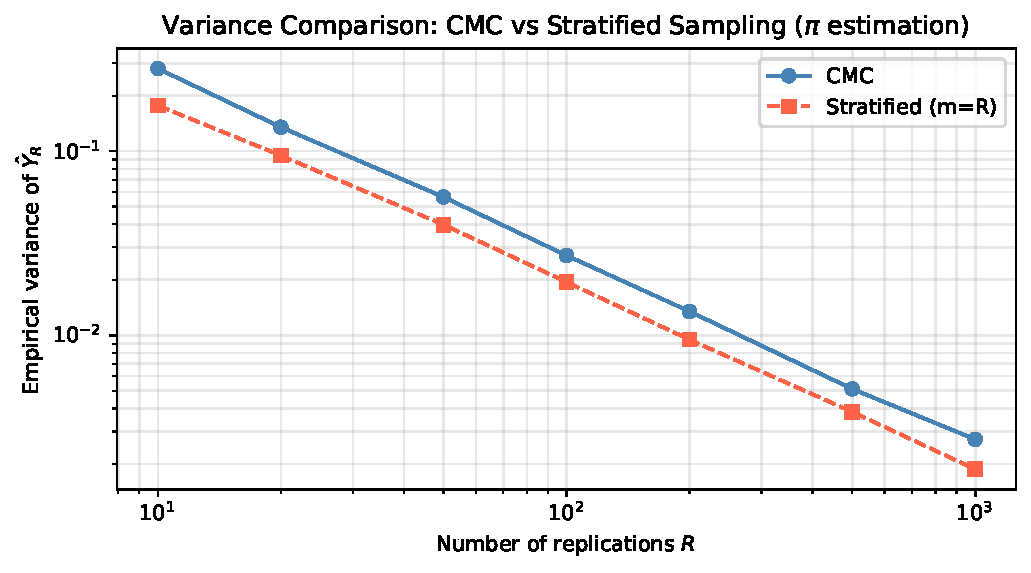
\includegraphics[width=0.75\textwidth]{fig_stratified_vs_cmc}
  \end{center}
  \vspace{-2mm}
  \small
  Stratified sampling reduces variance significantly -- the gap widens as $m$
  (number of strata) increases.
  Optimal allocation beats proportional, which beats CMC.
  Both converge to $\pi$ as $R \to \infty$, but with different rates.
\end{frame}

\begin{frame}{5.1.1 Optimal vs.\ Proportional Allocation}
  \begin{center}
    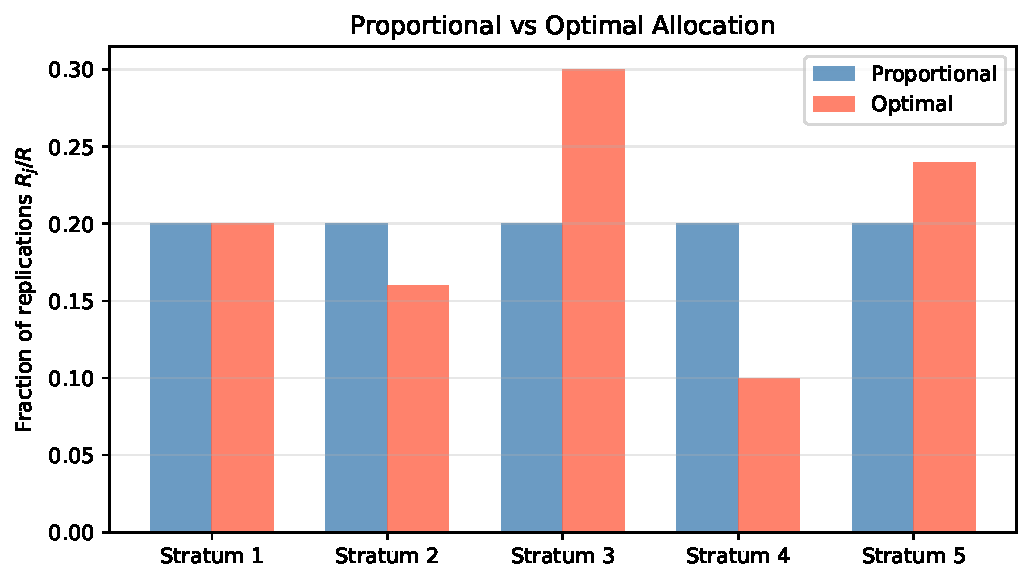
\includegraphics[width=0.72\textwidth]{fig_stratified_allocation}
  \end{center}
  \small
  Optimal allocation assigns more samples to strata with larger $\sigma_j$
  (within-stratum standard deviation), regardless of stratum probability $p_j$.
  For $Y = 4\sqrt{1-U^2}$, the rightmost stratum (steep curve near $U=1$)
  has by far the highest variability and receives the most replications.
\end{frame}

% ==============================================================================
\subsection{5.1.2 Antithetic Variates}
% ==============================================================================

\begin{frame}[allowframebreaks]{5.1.2 Antithetic Variates}

Antithetic variates reduce variance by generating pairs of estimates that
are \emph{negatively correlated}: when one overestimates $I$, the other
tends to underestimate it, so that their average cancels out the errors.

\begin{block}{The Antithetic Estimator}
  Instead of generating $R$ independent copies of $Y$, generate $R/2$ pairs
  $(Y_1^*, Y_1^*{}'), \ldots, (Y_{R/2}^*, Y_{R/2}^*{}')$ such that:
  \begin{itemize}
    \item $Y_i^* \overset{d}{=} Y$ and $Y_i^*{}' \overset{d}{=} Y$ (both have
          the correct marginal distribution),
    \item Pairs $(Y_{2i-1}^*, Y_{2i}^*)$ are i.i.d.\ (independent across pairs).
  \end{itemize}
  The antithetic estimator is:
  \[
    \hat{Y}_R^* = \frac{1}{R}\sum_{j=1}^R Y_j^*
    = \frac{1}{R/2}\sum_{i=1}^{R/2}\frac{Y_{2i-1}^* + Y_{2i}^*}{2}.
  \]
  Its variance compared to CMC (using (5.1.15) from the book):
  \[
    \mathrm{Var}(\hat{Y}_R^*) = \mathrm{Var}(\hat{Y}_R^{\mathrm{CMC}})
    \cdot\bigl(1 + \mathrm{Corr}(Y_1^*, Y_2^*)\bigr).
  \]
  Here $\mathrm{Corr}$ (correlation, ranging from $-1$ to $+1$) between the
  two members of a pair. If $\mathrm{Corr}(Y_1^*, Y_2^*) < 0$, variance decreases.
\end{block}

\framebreak

\begin{block}{Standard Construction: Complement in $[0,1]$}
  If $Y = k(U_1, \ldots, U_n)$ where $U_i \overset{\mathrm{iid}}{\sim} \mathcal{U}[0,1]$,
  define the antithetic pair via:
  \[
    Y_1^{\mathrm{anti}} = k(U_1, \ldots, U_n), \quad
    Y_2^{\mathrm{anti}} = k(1-U_1, \ldots, 1-U_n).
  \]
  Since $U_i$ and $1-U_i$ have the same marginal distribution ($\mathcal{U}[0,1]$),
  both $Y_1^{\mathrm{anti}}$ and $Y_2^{\mathrm{anti}}$ have the same distribution as $Y$.
\end{block}

\begin{block}{Theorem 5.1.13 and Corollary 5.1.14 -- When Antithetics Work}
  If $k(x_1, \ldots, x_n)$ is \emph{monotone} (meaning non-decreasing or
  non-increasing) in each variable $x_i$, then:
  \[
    \mathrm{Cov}\bigl(k(U_1,\ldots,U_n),\; k(1-U_1,\ldots,1-U_n)\bigr) \le 0.
  \]
  This guarantees a variance reduction. The proof relies on a fundamental
  inequality: if $k_1$ and $k_2$ are simultaneously monotone, then
  $\mathbb{E}[k_1(X)k_2(X)] \ge \mathbb{E}[k_1(X)]\mathbb{E}[k_2(X)]$.
\end{block}

\framebreak

\begin{exampleblock}{Example 5.1.13 -- Estimating $\mathbb{E}[e^U]$ with Antithetics}
  Let $Y = e^U$ where $U \sim \mathcal{U}[0,1]$.
  The antithetic pair is $Y^{\mathrm{anti}} = e^{1-U}$.
  The true value is $I = \mathbb{E}[e^U] = e - 1 \approx 1.7183$.

  \medskip
  \textbf{Variance of CMC:} $\mathrm{Var}(e^U) = \mathbb{E}[e^{2U}] - (e-1)^2
  = (e^2-1)/2 - (e-1)^2 \approx 0.242$.

  \medskip
  \textbf{Antithetic variance:} The average is $(e^U + e^{1-U})/2$.
  \[
    \mathrm{Var}\!\left(\frac{e^U+e^{1-U}}{2}\right) \approx 0.00474,
  \]
  a reduction factor of $0.242 / 0.00474 \approx 51$.

  \medskip
  This dramatic improvement occurs because $e^U$ and $e^{1-U}$ are strongly
  negatively correlated: when $U$ is large (making $e^U$ large),
  $1-U$ is small (making $e^{1-U}$ small), so the pair tends to cancel out errors.
\end{exampleblock}

\begin{alertblock}{Key Takeaway}
  Antithetic variates require essentially no extra computation: you generate
  one pair instead of one independent sample. The technique works best when
  the integrand $k$ is monotone. For non-monotone functions, antithetics may
  actually increase variance.
\end{alertblock}

\end{frame}

\begin{frame}[fragile]{5.1.2 Antithetic Variates -- Python Code}
\begin{lstlisting}[style=python]
import numpy as np

def antithetic_exp(R):
    """Estimate E[e^U], U~U[0,1], using antithetic variates."""
    U  = np.random.uniform(0, 1, R // 2)
    Y1 = np.exp(U)           # original
    Y2 = np.exp(1 - U)       # antithetic (complement)
    return np.mean((Y1 + Y2) / 2)

def antithetic_pi(R):
    """Estimate pi using antithetic variates: Y = 4*sqrt(1-U^2)."""
    U  = np.random.uniform(0, 1, R // 2)
    Y1 = 4 * np.sqrt(1 - U**2)
    Y2 = 4 * np.sqrt(1 - (1-U)**2)   # Y(1-U) is antithetic
    return np.mean((Y1 + Y2) / 2)

np.random.seed(42)
R = 100000
# E[e^U] = e - 1 ~ 1.71828
print(f"Antithetic E[e^U] = {antithetic_exp(R):.6f}  (true: {np.e-1:.6f})")
print(f"Antithetic pi     = {antithetic_pi(R):.6f}  (true: {np.pi:.6f})")

# Variance comparison: run 2000 repetitions of size 1000
cmc_vars  = np.var([np.mean(4*np.sqrt(1-np.random.uniform(0,1,1000)**2))
                    for _ in range(2000)])
anti_vars = np.var([antithetic_pi(1000) for _ in range(2000)])
print(f"CMC variance:       {cmc_vars:.6f}")
print(f"Antithetic variance:{anti_vars:.6f}")
print(f"Reduction:          {cmc_vars/anti_vars:.1f}x")
\end{lstlisting}
\end{frame}

\begin{frame}{5.1.2 Antithetic Variates -- Illustration}
  \begin{center}
    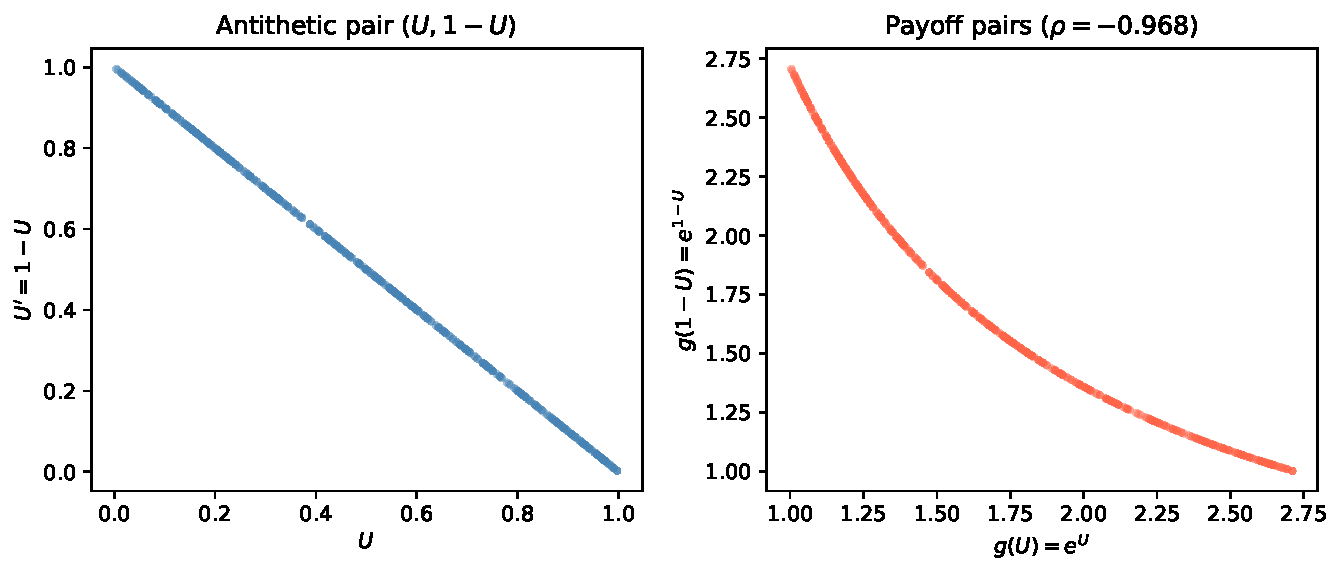
\includegraphics[width=0.85\textwidth]{fig_antithetic}
  \end{center}
  \small
  Left: The pair $(U, 1-U)$ is perfectly negatively correlated.
  Right: The corresponding payoffs $k(U)$ and $k(1-U)$ also show strong negative correlation,
  so their average has much lower variance than either one alone.
\end{frame}

% ==============================================================================
\subsection{5.1.3 Common Random Numbers}
% ==============================================================================

\begin{frame}[allowframebreaks]{5.1.3 Common Random Numbers (CRN)}

Common random numbers (CRN) is a technique for \emph{comparing two systems}:
instead of estimating a single $\mathbb{E}[Y]$, we want to estimate the difference
$\Delta = \mathbb{E}[Y_1] - \mathbb{E}[Y_2]$ between outputs of two system configurations.
By using the \emph{same} random numbers to drive both simulations, we induce
positive correlation between $Y_1$ and $Y_2$, which reduces the variance of
the difference estimator.

\begin{block}{CRN Estimator}
  Use the same random stream $U$ to simulate both systems. Generate $R$ pairs:
  \[
    \hat{\Delta}_R^{\mathrm{CRN}} = \frac{1}{R}\sum_{j=1}^R(Y_{1,j} - Y_{2,j}),
  \]
  where $(Y_{1,j}, Y_{2,j})$ are the outputs of systems 1 and 2 using the
  same random input $U_j$. The variance is:
  \[
    \mathrm{Var}(\hat{\Delta}_R^{\mathrm{CRN}})
    = \frac{\mathrm{Var}(Y_1) + \mathrm{Var}(Y_2) - 2\mathrm{Cov}(Y_1,Y_2)}{R}.
  \]
  CRN reduces variance when $\mathrm{Cov}(Y_1, Y_2) > 0$, which is the common
  case when both systems respond monotonically to the same random input.
\end{block}

\framebreak

\textbf{Why CRN induces positive covariance:}
If both $Y_1 = k_1(U)$ and $Y_2 = k_2(U)$ are non-decreasing functions of
the same input $U$, then Theorem 5.1.13 gives
$\mathrm{Cov}(k_1(U), k_2(U)) \ge 0$.

\begin{exampleblock}{Example -- Scheduling Problem (Example 5.1.20)}
  Consider two scheduling policies for a queue (FCFS vs.\ LCFS ordering).
  We want to estimate the difference in expected throughput $\Delta$.
  Using CRN:
  \begin{itemize}
    \item The same sequence of service times and inter-arrival times is
          fed to both policies in each replication.
    \item When service times happen to be long (bad run), both policies
          suffer similarly, so $Y_1 - Y_2$ is stable.
    \item Result from book: for $R=1000$, variance reduced by factor
          $\approx 22.5\times$ compared to independent replications.
  \end{itemize}
\end{exampleblock}

\begin{alertblock}{Synchronisation Warning}
  When systems have different structures (different number of events,
  different branching), naive use of CRN may fail to induce positive
  correlation. Careful mapping of the random number stream to the same
  logical variable in both systems (called \emph{synchronisation}) is required.
\end{alertblock}

\end{frame}

% ==============================================================================
\subsection{5.1.4 Ratios of Expectations}
% ==============================================================================

\begin{frame}[allowframebreaks]{5.1.4 Ratios of Expectations}

Sometimes the quantity of interest is itself a ratio of two expectations:
$I = I^{(1)} / I^{(2)}$ where $I^{(1)} = \mathbb{E}[Y^{(1)}]$ and
$I^{(2)} = \mathbb{E}[Y^{(2)}]$. This arises, for example, in conditional
expectations and self-normalised importance sampling.

\begin{block}{Ratio Estimator}
  Generate $R$ i.i.d.\ pairs $(Y_1^{(1)}, Y_1^{(2)}), \ldots, (Y_R^{(1)}, Y_R^{(2)})$
  and define:
  \[
    \hat{Y}_R^{\mathrm{RoE}} = \frac{\sum_{i=1}^R Y_i^{(1)}}{\sum_{i=1}^R Y_i^{(2)}}
    = \frac{\hat{Y}_R^{(1)}}{\hat{Y}_R^{(2)}},
  \]
  where $\hat{Y}_R^{(1)}$ and $\hat{Y}_R^{(2)}$ are the sample means.
  This estimator is \emph{biased} (the ratio of sample means is not the same as
  the sample mean of ratios), but it is \emph{consistent} (converges to $I$ as $R \to \infty$).
\end{block}

\framebreak

\begin{block}{Asymptotic Variance via the Delta Method}
  The \emph{delta method} (also called the propagation of uncertainty formula)
  approximates the variance of a function of sample means. For the ratio estimator:
  \[
    (\varsigma^{\mathrm{RoE}})^2 = \frac{I^{(1)}}{I^{(2)}}
    \left[\frac{\Sigma_{\mathbf{Y}}(1,1)}{(I^{(1)})^2}
          - \frac{2\,\Sigma_{\mathbf{Y}}(1,2)}{I^{(1)}I^{(2)}}
          + \frac{\Sigma_{\mathbf{Y}}(2,2)}{(I^{(2)})^2}\right]^{1/2},
  \]
  where $\Sigma_{\mathbf{Y}}(i,j) = \mathrm{Cov}(Y^{(i)}, Y^{(j)})$.
  By choosing the joint distribution of $(Y^{(1)}, Y^{(2)})$ to induce positive
  covariance $\Sigma_{\mathbf{Y}}(1,2)$, we can reduce the variance of the ratio
  estimator. This is the connection to common random numbers (CRN).
\end{block}

\begin{alertblock}{Application: Self-Normalised Importance Sampling}
  Self-normalised IS (see Section 5.1.7) uses a ratio estimator when the
  normalisation constant of a distribution is unknown. The ratio estimator
  is consistent and the delta method provides the confidence interval.
\end{alertblock}

\end{frame}

% ==============================================================================
\subsection{5.1.5 Control Variates}
% ==============================================================================

\begin{frame}[allowframebreaks]{5.1.5 Control Variates}

A control variate is a random variable $X$ that is \emph{correlated} with
the output $Y$ and has a \emph{known mean} $\mu_X = \mathbb{E}[X]$.
The idea is to correct the CMC estimate $\hat{Y}_R$ by subtracting the
observed deviation of $X$ from its known mean.

\begin{block}{The Control Variate Estimator}
  Given primary output $Y$ with $I = \mathbb{E}[Y]$ (unknown), control variate
  $X$ with $\mu_X = \mathbb{E}[X]$ (known), and scalar coefficient $c$ (c for control):
  \[
    \hat{Y}_R^{\mathrm{cv}} = \hat{Y}_R + c\,(\hat{X}_R - \mu_X),
  \]
  where $\hat{Y}_R = \frac{1}{R}\sum_i Y_i$ and $\hat{X}_R = \frac{1}{R}\sum_i X_i$
  are sample means from the same $R$ replications.

  This estimator is \emph{unbiased} because $\mathbb{E}[\hat{X}_R - \mu_X] = 0$.
  Its variance is:
  \[
    \mathrm{Var}(\hat{Y}_R^{\mathrm{cv}}) = \frac{1}{R}\bigl[\mathrm{Var}(Y)
    + c^2\,\mathrm{Var}(X) + 2c\,\mathrm{Cov}(X,Y)\bigr].
  \]
\end{block}

\framebreak

\begin{block}{Optimal Coefficient $c^*$ and Resulting Variance}
  Minimising the variance over $c$ gives:
  \[
    c^* = -\frac{\mathrm{Cov}(X,Y)}{\mathrm{Var}(X)}.
  \]
  Here $\mathrm{Cov}(X,Y)$ (covariance of $X$ and $Y$, measuring how they move together)
  divided by $\mathrm{Var}(X)$ (variance of $X$) gives the regression slope of $Y$ on $X$.
  The optimal variance is:
  \[
    \mathrm{Var}(\hat{Y}_R^{\mathrm{cv},*}) = \frac{\mathrm{Var}(Y)}{R}(1 - \rho^2),
  \]
  where $\rho$ (rho) $= \mathrm{Corr}(X,Y)$ is the correlation between $X$ and $Y$.
  The \emph{variance reduction factor} is $1/(1-\rho^2)$, which is always $\ge 1$.
\end{block}

\begin{alertblock}{How to Read This}
  If $\rho^2 = 0.9$ (strongly correlated), the variance is reduced by factor
  $1/(1-0.9) = 10$. If $\rho = 0$ (uncorrelated), no reduction occurs.
  The control variate works by ``explaining away'' the variability in $Y$ that
  is linearly predictable from $X$.
\end{alertblock}

\framebreak

\begin{block}{Estimated Coefficient (Pilot Simulation)}
  In practice, $c^* = -\mathrm{Cov}(X,Y)/\mathrm{Var}(X)$ is unknown.
  Run $R'$ pilot replications to estimate:
  \[
    \hat{c} = -\frac{\hat{S}_{XY}^2}{\hat{S}_X^2},
  \]
  where $\hat{S}_{XY}^2 = \frac{1}{R'-1}\sum_{i=1}^{R'}(X_i - \bar{X})(Y_i - \bar{Y})$
  is the sample covariance and $\hat{S}_X^2$ is the sample variance of $X$.
  Then run $R$ main replications and apply:
  $\hat{Y}_R^{\mathrm{cv}} = \hat{Y}_R + \hat{c}(\hat{X}_R - \mu_X)$.
\end{block}

\begin{exampleblock}{Example 5.1.24 -- $\pi$ with Control Variates}
  Estimate $I = \pi$ using $Y = 4\sqrt{1-U^2}$, $U \sim \mathcal{U}[0,1]$.
  \begin{itemize}
    \item \textbf{Control variate 1:} $X = 1-U$ with $\mu_X = \mathbb{E}[1-U] = 1/2$.\\
          $\rho \approx 0.528$, variance reduction $\approx 1.4\times$.
    \item \textbf{Control variate 2:} $X = \mathbf{1}(U + (1-U) > \sqrt{2})$, $\mu_X$ known.\\
          $1-\rho^2 = 0.242$, variance reduction $\approx 4\times$.
    \item \textbf{Control variate 3:} degree-4 polynomial in $U$ tuned to $Y$.\\
          $1-\rho^2 = 0.0000860$, variance reduction $\approx 11{,}630\times$!
  \end{itemize}
  The lesson: a cleverly chosen control variate can achieve enormous reductions.
  The more $X$ ``explains'' the variability of $Y$ (high $\rho^2$), the better.
\end{exampleblock}

\end{frame}

\begin{frame}[fragile]{5.1.5 Control Variates -- Python Code}
\begin{lstlisting}[style=python]
import numpy as np

def control_variate_pi(R, R_pilot=1000):
    """Estimate pi using control variate X = 1-U, E[X] = 0.5."""
    # Pilot: estimate c* = -Cov(X,Y)/Var(X)
    U_p = np.random.uniform(0, 1, R_pilot)
    Y_p = 4 * np.sqrt(1 - U_p**2)   # primary output
    X_p = 1 - U_p                    # control variate (E[X] = 0.5)
    cov_mat = np.cov(X_p, Y_p, ddof=1)
    c_hat = -cov_mat[0, 1] / cov_mat[0, 0]
    rho   = np.corrcoef(X_p, Y_p)[0, 1]
    print(f"  Estimated c* = {c_hat:.4f},  rho = {rho:.4f}")
    print(f"  Theoretical reduction = {1/(1-rho**2):.2f}x")

    # Main simulation
    U = np.random.uniform(0, 1, R)
    Y = 4 * np.sqrt(1 - U**2)
    X = 1 - U
    Y_cv = Y + c_hat * (X - 0.5)    # control variate adjustment
    return np.mean(Y_cv), np.std(Y_cv) / np.sqrt(R)

np.random.seed(42)
est, se = control_variate_pi(R=100000)
print(f"CV estimate:  {est:.6f} +/- {1.96*se:.6f}")
print(f"True pi:      {np.pi:.6f}")
\end{lstlisting}
\end{frame}

\begin{frame}{5.1.5 Control Variates -- Regression View}
  \begin{center}
    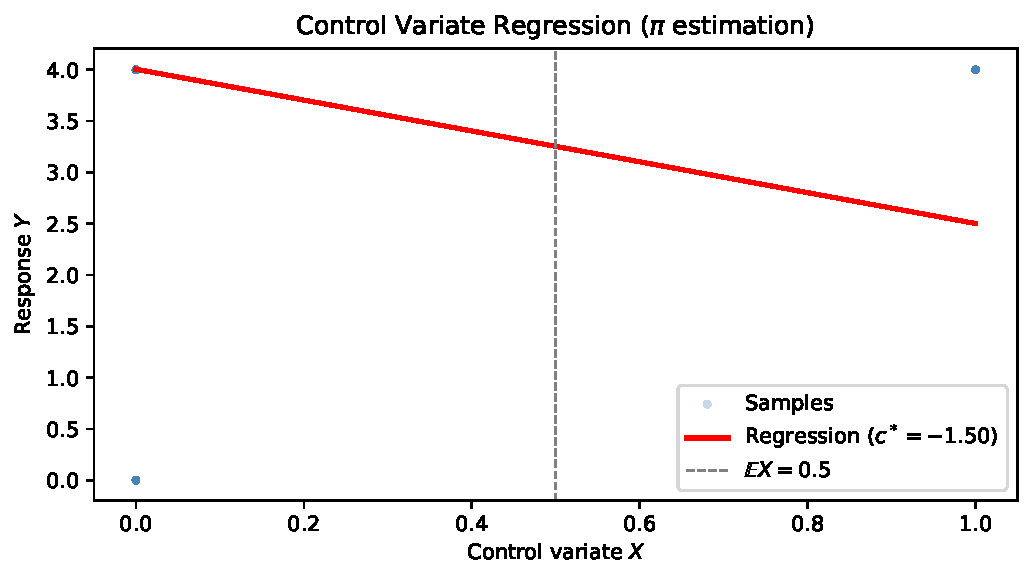
\includegraphics[width=0.72\textwidth]{fig_control_variates}
  \end{center}
  \small
  The control variate estimator fits a regression line through the $(X, Y)$
  scatter plot. The optimal coefficient $c^* = -\mathrm{Cov}(X,Y)/\mathrm{Var}(X)$
  is the negative of the regression slope. The residuals from this regression
  have lower variance than $Y$ itself -- that is exactly the variance reduction.
\end{frame}

% ==============================================================================
\subsection{5.1.6 Conditional Monte Carlo}
% ==============================================================================

\begin{frame}[allowframebreaks]{5.1.6 Conditional Monte Carlo (Rao-Blackwell)}

Conditional Monte Carlo (also called the Rao-Blackwell method) exploits the
structure of a problem by computing a conditional expectation analytically
instead of simulating it. If we can compute $c(x) = \mathbb{E}[Y \mid X = x]$
in closed form, then $c(X)$ is a better estimator of $I = \mathbb{E}[Y]$
than $Y$ itself.

\begin{block}{The Conditional Estimator}
  Given $I = \mathbb{E}[Y] = \mathbb{E}[c(X)]$ where $c(x) = \mathbb{E}[Y \mid X=x]$,
  generate $X_1, \ldots, X_R$ i.i.d.\ copies of $X$ and compute:
  \[
    \hat{Y}_R^{\mathrm{cond}} = \frac{1}{R}\sum_{j=1}^R c(X_j).
  \]
  This estimator uses the analytically computed conditional mean $c(X_j)$
  instead of one noisy sample $Y_j$ per replication.
\end{block}

\framebreak

\begin{block}{Rao-Blackwell Theorem: Conditioning Always Reduces Variance}
  By the law of total variance:
  \[
    \mathrm{Var}(Y) = \underbrace{\mathbb{E}[\mathrm{Var}(Y\mid X)]}_{\ge\, 0}
    + \mathrm{Var}(\mathbb{E}[Y\mid X]) = \mathbb{E}[\mathrm{Var}(Y\mid X)] + \mathrm{Var}(c(X)).
  \]
  Since $\mathbb{E}[\mathrm{Var}(Y\mid X)] \ge 0$, we have:
  \[
    \mathrm{Var}(c(X)) \le \mathrm{Var}(Y).
  \]
  This is strict unless $Y = c(X)$ almost surely (i.e., $Y$ is already
  a deterministic function of $X$).
\end{block}

\begin{exampleblock}{Example 5.1.29 -- $\pi$ via Conditional MC}
  We estimate $\pi$ via the quarter-circle:
  $Y = 4\cdot\mathbf{1}(U_1^2 + U_2^2 \le 1)$ where $U_1, U_2 \sim \mathcal{U}[0,1]$.
  Condition on $X = U_1$:
  \[
    c(x) = \mathbb{E}[Y \mid U_1 = x]
    = 4\,\mathbb{P}(U_2 \le \sqrt{1-x^2}) = 4\sqrt{1-x^2}.
  \]
  The conditional estimator is just:
  $\hat{Y}_R^{\mathrm{cond}} = \frac{4}{R}\sum_{i=1}^R\sqrt{1-U_i^2}$.
  \begin{itemize}
    \item $\mathrm{Var}(\hat{Y}_R^{\mathrm{CMC}}) = 2.697/R$
    \item $\mathrm{Var}(\hat{Y}_R^{\mathrm{cond}}) = 0.797/R$
    \item Reduction factor: $\approx 3.38\times$
  \end{itemize}
\end{exampleblock}

\end{frame}

\begin{frame}{5.1.6 Conditional MC -- Variance Comparison}
  \begin{center}
    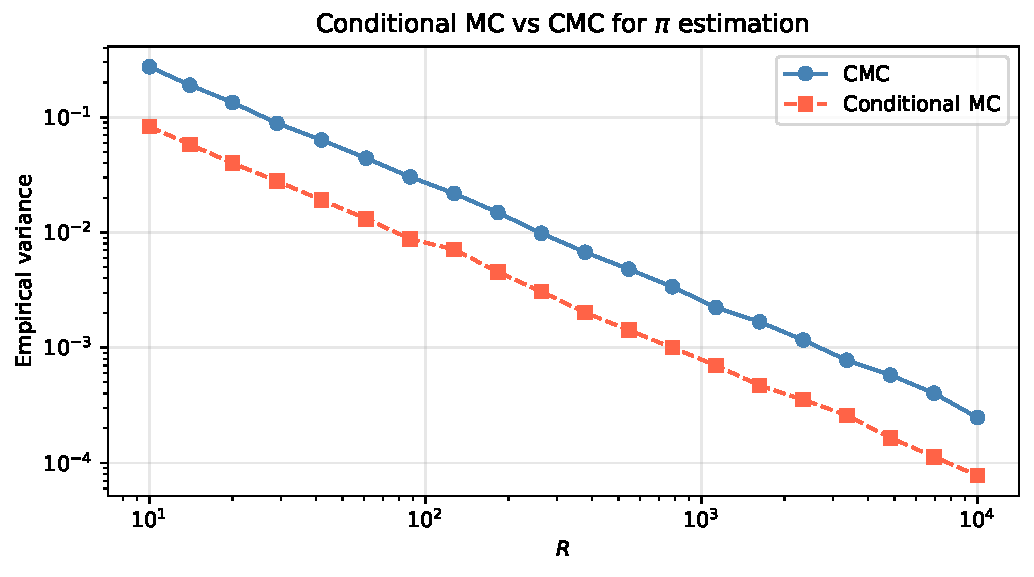
\includegraphics[width=0.72\textwidth]{fig_conditional_mc}
  \end{center}
  \small
  The conditional MC estimator uses the analytically computed $c(U_1) = 4\sqrt{1-U_1^2}$
  instead of the noisy indicator $4\cdot\mathbf{1}(U_1^2+U_2^2\le 1)$.
  Both converge at rate $1/R$, but the conditional estimator has a smaller constant.
\end{frame}

% ==============================================================================
\subsection{5.1.7 Importance Sampling}
% ==============================================================================

\begin{frame}[allowframebreaks]{5.1.7 Importance Sampling -- The Change-of-Measure Idea}

Importance sampling (IS) is a powerful technique that allows us to estimate
$I = \int k(x)f(x)\,dx = \mathbb{E}_f[k(X)]$ by sampling from a different
(easier or better-suited) distribution $\tilde{f}$ instead of $f$.
The key insight is that any expectation under $f$ can be rewritten as an
expectation under $\tilde{f}$ by multiplying by the ratio $f(x)/\tilde{f}(x)$.

\begin{block}{Importance Sampling Identity}
  Let $\tilde{f}$ (f-tilde, the \emph{proposal} or \emph{importance} density)
  satisfy $\tilde{f}(x) > 0$ wherever $k(x)f(x) \ne 0$.
  Define the \emph{likelihood ratio} (also called importance weight):
  \[
    L(x) = \frac{f(x)}{\tilde{f}(x)}.
  \]
  Then:
  \[
    I = \int_E k(x)\frac{f(x)}{\tilde{f}(x)}\tilde{f}(x)\,dx
      = \mathbb{E}_{\tilde{f}}\!\left[k(\tilde{X})\cdot L(\tilde{X})\right],
  \]
  where $\tilde{X} \sim \tilde{f}$ (tilde-X is sampled from the proposal density).
\end{block}

\framebreak

\begin{block}{Importance Sampling Estimator}
  Generate $\tilde{X}_1, \ldots, \tilde{X}_R \overset{\mathrm{iid}}{\sim} \tilde{f}$
  and compute:
  \[
    \hat{Y}_R^{\mathrm{IS}} = \frac{1}{R}\sum_{j=1}^R k(\tilde{X}_j)\,\frac{f(\tilde{X}_j)}{\tilde{f}(\tilde{X}_j)}.
  \]
  Each sample is \emph{weighted} by the likelihood ratio $L(\tilde{X}_j) = f(\tilde{X}_j)/\tilde{f}(\tilde{X}_j)$
  to correct for the fact that we sampled from $\tilde{f}$ rather than $f$.
\end{block}

\begin{block}{Variance of IS Estimator (Proposition 5.1.33)}
  The IS estimator is unbiased and strongly consistent. By the CLT:
  \[
    \sqrt{R}(\hat{Y}_R^{\mathrm{IS}} - I) \xrightarrow{\mathcal{D}} \mathcal{N}(0, \varsigma^2),
  \]
  where:
  \[
    \varsigma^2 = \int_E \!\left(k(x)\frac{f(x)}{\tilde{f}(x)}\right)^2\!\tilde{f}(x)\,dx - I^2
    = \mathrm{Var}_{\tilde{f}}\!\left[k(\tilde{X})L(\tilde{X})\right].
  \]
  To reduce variance, choose $\tilde{f}$ so that the weighted integrand
  $k(x)f(x)/\tilde{f}(x)$ is as \emph{flat} (constant) as possible.
\end{block}

\framebreak

\begin{block}{Optimal Proposal Distribution (Zero-Variance IS)}
  The variance $\varsigma^2$ is minimised at $\varsigma^2 = 0$ by the
  \emph{zero-variance proposal}:
  \[
    \tilde{f}^*(x) = \frac{|k(x)|f(x)}{\int_E |k(x)|f(x)\,dx}
    = \frac{|k(x)|f(x)}{I'}
  \]
  (proportional to the absolute integrand), because then
  $k(x)f(x)/\tilde{f}^*(x) = I'$ is constant.

  \textbf{Caveat:} This requires knowing the integral $I'$ (essentially knowing $I$),
  so it cannot be used directly. However, it guides the choice of $\tilde{f}$:
  the proposal should be large where $|k(x)|f(x)$ is large, i.e., concentrate
  samples in the most important regions.
\end{block}

\begin{exampleblock}{Example 5.1.34 -- IS for a Cauchy Tail Probability}
  Estimate $I = \mathbb{P}(X > 2)$ where $X$ has a Cauchy distribution:
  $f(x) = 1/(\pi(1+x^2))$.
  The true value is $I = 1/2 - \arctan(2)/\pi \approx 0.14758$.
  \begin{itemize}
    \item \textbf{CMC:} $\mathrm{Var}(\hat{Y}_R^{\mathrm{CMC}}) = I(1-I)/R = 0.1258/R$.
    \item \textbf{IS} with proposal $\tilde{f}(x) = \frac{2}{x^2}\mathbf{1}(x>2)$
          (a Pareto-type density concentrated on $(2,\infty)$):
          Simulating $\tilde{X} \sim \tilde{f}$ via the inverse CDF: $\tilde{X} = 2/U$
          where $U \sim \mathcal{U}[0,1]$.
    \item IS variance: $\mathrm{Var}(\hat{Y}_R^{\mathrm{IS}}) = 9.55\times 10^{-5}/R$.
    \item Reduction: $0.1258 / (9.55\times 10^{-5}) \approx 1317\times$.
  \end{itemize}
\end{exampleblock}

\end{frame}

\begin{frame}[allowframebreaks]{5.1.7 IS for Rare Events -- Normal Tail}

\begin{exampleblock}{Example 5.1.36 -- IS for $\mathbb{P}(Z > 4)$, $Z\sim\mathcal{N}(0,1)$}
  The standard normal tail probability $I = \mathbb{P}(Z > 4) \approx 3.167\times 10^{-5}$
  is very small (rare event). CMC is almost useless: most samples give $Y = 0$.

  \medskip
  \textbf{Idea:} Shift the proposal to $\tilde{f} = \mathcal{N}(\theta, 1)$
  (normal with mean $\theta$, shifted towards the rare region).
  The likelihood ratio is:
  \[
    L(z) = \frac{\phi_{0,1}(z)}{\phi_{\theta,1}(z)} = e^{-\theta z + \theta^2/2},
  \]
  where $\phi_{0,1}$ is the standard normal density (phi sub 0-1) and
  $\phi_{\theta,1}$ is the density of $\mathcal{N}(\theta,1)$.
  The IS estimator becomes:
  \[
    \hat{Y}_R^{\mathrm{IS},\theta} = \frac{1}{R}\sum_{i=1}^R \mathbf{1}(\tilde{Z}_i > 4)\,
    e^{-\theta\tilde{Z}_i + \theta^2/2}, \quad \tilde{Z}_i \sim \mathcal{N}(\theta,1).
  \]
\end{exampleblock}

\framebreak

\textbf{Numerical comparison} for $I = \mathbb{P}(Z > 4)$:
\begin{center}\small
  \begin{tabular}{lccc}
    \toprule
    Proposal $\theta$ & Estimate ($R=10^5$) & $\mathrm{Var}/R$ & Reduction \\
    \midrule
    0 (CMC) & varies wildly & $3.17\times 10^{-5}$ & $1\times$ \\
    $\theta = 2$ & $\approx 3.2\times 10^{-5}$ & $5.6\times 10^{-8}$ & $566\times$ \\
    $\theta = 4$ & $\approx 3.2\times 10^{-5}$ & $3.6\times 10^{-8}$ & $879\times$ \\
    $\theta = 4.2256$ (CE opt.) & $\approx 3.2\times 10^{-5}$ & $4.5\times 10^{-9}$ & $7000\times$ \\
    \bottomrule
  \end{tabular}
\end{center}

The choice $\theta = 4$ (shifting the proposal mean to the rare-event boundary)
gives nearly $900\times$ improvement. The cross-entropy optimal $\theta^* = 4.2256$
does even better (Section 5.1.8).

\begin{alertblock}{How to Read This}
  IS for rare events works by moving the entire proposal distribution to
  where the rare event lives. Samples are then drawn mostly from the
  region $Z > 4$, and each is downweighted by $e^{-\theta Z + \theta^2/2}$
  to correct for the fact that we over-sampled that region.
\end{alertblock}

\end{frame}

\begin{frame}[fragile]{5.1.7 Importance Sampling -- Python Code}
\begin{lstlisting}[style=python]
import numpy as np
from scipy.stats import norm

def IS_normal_tail(theta, R=100000):
    """Estimate P(Z>4), Z~N(0,1), using IS with N(theta,1) proposal."""
    Z = np.random.normal(theta, 1, R)
    # Log likelihood ratio: log[phi(z;0,1)/phi(z;theta,1)]
    log_LR = -theta * Z + theta**2 / 2
    Y_IS   = (Z > 4).astype(float) * np.exp(log_LR)
    est    = np.mean(Y_IS)
    var    = np.var(Y_IS, ddof=1) / R
    return est, var

np.random.seed(42)
true_I = 1 - norm.cdf(4)
print(f"True P(Z>4) = {true_I:.4e}")
print()
for theta in [0, 2, 4, 4.2256]:
    est, var = IS_normal_tail(theta)
    label = "(CMC)" if theta == 0 else ""
    reduction = true_I * (1 - true_I) / (R := 100000) / var if var > 0 else float('inf')
    print(f"theta={theta:.4f} {label:6s}: est={est:.3e}, "
          f"var/R={var:.3e}, reduction={true_I*(1-true_I)/var:.0f}x")
\end{lstlisting}
\end{frame}

\begin{frame}{5.1.7 IS Proposal Distributions}
  \begin{center}
    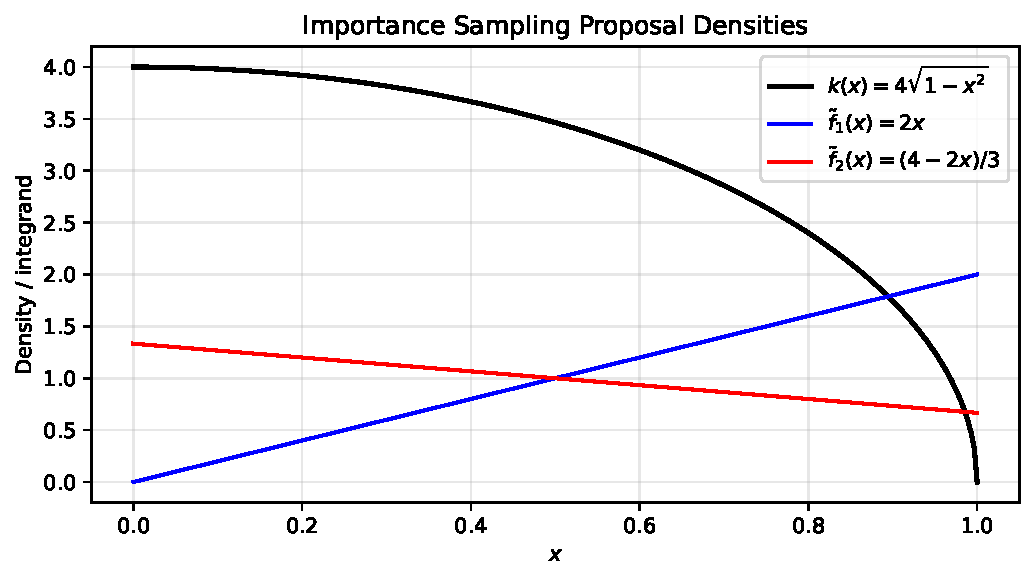
\includegraphics[width=0.72\textwidth]{fig_IS_proposals}
  \end{center}
  \small
  The optimal proposal $\tilde{f}^*(x) \propto |k(x)|f(x)$ should closely
  match the shape of the absolute integrand. Among competing proposals,
  the one whose shape best matches $k(x)f(x)$ achieves lower variance.
  A proposal that is too light in the tails inflates variance; too heavy
  causes high-variance weights.
\end{frame}

\begin{frame}{5.1.7 IS for Rare Events: $\mathbb{P}(Z>4)$}
  \begin{center}
    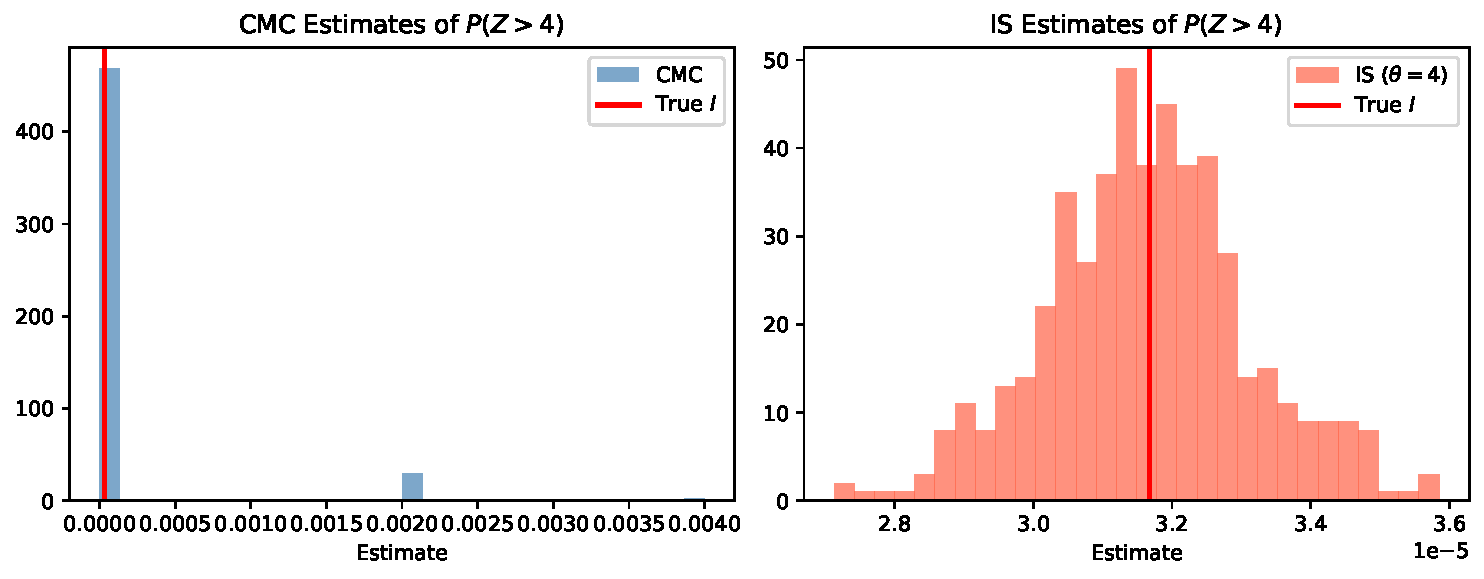
\includegraphics[width=0.82\textwidth]{fig_IS_rare_event}
  \end{center}
  \small
  Top: CMC estimates are mostly exactly 0 (the event $Z>4$ almost never
  occurs in random standard normal draws). Bottom: IS with $\tilde{f} = \mathcal{N}(4,1)$
  concentrates all samples in the relevant region $Z>4$, giving consistent
  and low-variance estimates.
\end{frame}

\begin{frame}[allowframebreaks]{5.1.7 Self-Normalised Importance Sampling}

When the normalisation constants of both the target $f$ and the proposal $\tilde{f}$
are unknown (a common situation in Bayesian statistics), we can still form a
consistent estimator using a ratio (Rao-Blackwell) approach.

\begin{block}{Self-Normalised IS Estimator}
  Suppose $f(x) = c \cdot f_0(x)$ and $\tilde{f}(x) = \tilde{c}\cdot\tilde{f}_0(x)$
  with unknown constants. Define unnormalised weights $w(x) = f_0(x)/\tilde{f}_0(x)$.
  Then:
  \[
    I = \frac{\mathbb{E}_{\tilde{f}}[k(\tilde{X})w(\tilde{X})]}{\mathbb{E}_{\tilde{f}}[w(\tilde{X})]},
  \]
  estimated by the ratio:
  \[
    \hat{Y}_R^{\mathrm{SN}} = \frac{\sum_{i=1}^R k(\tilde{X}_i)w(\tilde{X}_i)}
                                   {\sum_{i=1}^R w(\tilde{X}_i)}
    = \sum_{i=1}^R k(\tilde{X}_i)\,w_i^{\mathrm{norm}},
  \]
  where $w_i^{\mathrm{norm}} = w(\tilde{X}_i)/\sum_j w(\tilde{X}_j)$ are the
  \emph{normalised weights} (each between 0 and 1, summing to 1).
  This estimator is \emph{biased} but consistent (bias $\to 0$ as $R\to\infty$).
\end{block}

\framebreak

\begin{block}{Exponential Change of Measure (Rare-Event Efficiency)}
  For sum $S_n = X_1 + \cdots + X_n$ of i.i.d.\ random variables with mean $\mu$
  (mu, the expected value) and cumulant generating function
  $\kappa(\theta) = \log\mathbb{E}[e^{\theta X}]$ (kappa of theta):
  Define the \emph{exponentially twisted} density $f_\theta(x) = e^{\theta x - \kappa(\theta)}f(x)$.
  Under $\mathbb{P}_\theta$, we have $\mathbb{E}_\theta[X_1] = \kappa'(\theta)$.
  Choose $\theta = \theta_0$ such that $\kappa'(\theta_0) = \mu + \varepsilon$
  (i.e., the twisted mean equals the rare-event threshold).
  The IS estimator for $I(n) = \mathbb{P}(S_n > n(\mu+\varepsilon))$ becomes:
  \[
    \hat{Y}_R^{\theta_0} = \frac{1}{R}\sum_{i=1}^R
    \mathbf{1}_{S_n^{(i)} > n(\mu+\varepsilon)}\,
    e^{-\theta_0 S_n^{(i)} + n\kappa(\theta_0)},
  \]
  and this estimator is \emph{logarithmically efficient} (the relative error
  does not explode as the event becomes rarer).
\end{block}

\end{frame}

\begin{frame}{5.1.7 Self-Normalised IS Weights}
  \begin{center}
    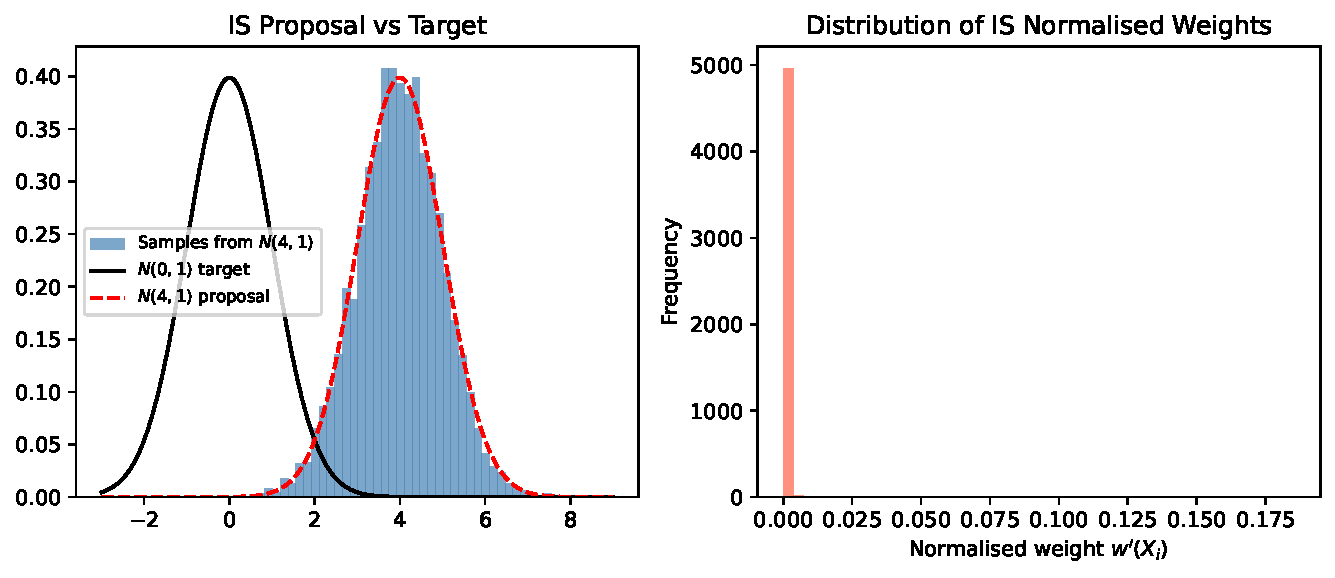
\includegraphics[width=0.82\textwidth]{fig_snIS_weights}
  \end{center}
  \small
  Using a proposal $\mathcal{N}(4,1)$ concentrates samples in the rare region $Z>4$.
  The normalised weights $w_i^{\mathrm{norm}} = w(\tilde{X}_i)/\sum_j w(\tilde{X}_j)$
  are well-spread (no single sample dominates), ensuring a stable estimate.
  Poor proposals lead to degenerate weight distributions where one or two
  samples carry almost all the weight.
\end{frame}

% ==============================================================================
\subsection{5.1.8 Cross-Entropy Method}
% ==============================================================================

\begin{frame}[allowframebreaks]{5.1.8 The Cross-Entropy Method -- Motivation}

The cross-entropy (CE) method provides a systematic procedure to find the
\emph{optimal IS proposal} from a parametric family $\{\tilde{f}_\theta : \theta \in \Theta\}$.
Rather than choosing $\theta$ by hand, CE adapts $\theta$ iteratively towards
the parameter that minimises the KL divergence from the ideal (zero-variance) proposal.

\begin{block}{KL Divergence and Optimal Parameter}
  The \emph{Kullback-Leibler (KL) divergence} (also called cross-entropy loss)
  from the zero-variance proposal $g^*(x) = k(x)f(x)/I$ to $\tilde{f}_\theta$ is:
  \[
    D_{\mathrm{KL}}(g^* \| \tilde{f}_\theta)
    = \int g^*(x)\log\frac{g^*(x)}{\tilde{f}_\theta(x)}\,dx.
  \]
  Minimising this over $\theta$ (theta, the parameter vector of the proposal family)
  is equivalent to maximising:
  \[
    \theta^* = \arg\max_\theta \mathbb{E}_f\!\left[k(X)\log\tilde{f}_\theta(X)\right].
  \]
  This can be estimated from $M$ samples $(X_1,\ldots,X_M)$ from $f$ as:
  \[
    \hat{\theta}^* = \arg\max_\theta \frac{1}{M}\sum_{i=1}^M k(X_i)\log\tilde{f}_\theta(X_i).
  \]
\end{block}

\framebreak

\begin{block}{CE for Rare Event Estimation: Iterative Algorithm}
  For $I = \mathbb{P}_f(h(\mathbf{X}) \ge \gamma)$ (probability that performance
  $h$ exceeds threshold $\gamma$, where $h$ (h) is the performance function
  and $\gamma$ (gamma) is the target level):

  \textbf{Initialise:} $\theta_0' = $ initial parameter (e.g., mean of $f$);
  $\rho$ (rho) $\in (0,1)$ is the quantile level (e.g., $\rho = 0.05$);
  $\alpha$ (alpha) $\in (0,1)$ is a smoothing factor.

  \textbf{Iterate} for $t = 1, 2, \ldots$:
  \begin{enumerate}
    \item \textbf{Sample:} Draw $X_1,\ldots,X_M \overset{\mathrm{iid}}{\sim} \tilde{f}_{\theta_{t-1}'}$.
    \item \textbf{Update level:} $\gamma_t = (1-\rho)$-quantile of $h(X_1),\ldots,h(X_M)$.
    \item \textbf{Update parameter:}
      \[
        \theta_t' = \arg\max_\theta \frac{1}{M}\sum_{i=1}^M
        \mathbf{1}(h(X_i)\ge\gamma_t)\,L(X_i; f, \tilde{f}_{\theta_{t-1}'})\,\log\tilde{f}_\theta(X_i).
      \]
    \item \textbf{Smooth:} $\theta_t' \leftarrow \alpha\theta_t' + (1-\alpha)\theta_{t-1}'$.
    \item \textbf{Stop} when $\gamma_t \ge \gamma$.
  \end{enumerate}

  \textbf{Final IS estimate:} Generate $R$ samples from $\tilde{f}_{\theta_T'}$
  and compute $\hat{Y}_R^{\mathrm{CE}} = \frac{1}{R}\sum_i \mathbf{1}(h(X_i)>\gamma)\,L(X_i)$.
\end{block}

\framebreak

\begin{block}{CE Update for Normal Family $\tilde{f}_\theta = \mathcal{N}(\mu, \sigma^2)$}
  For the one-dimensional normal family with parameter $\theta = \mu$ (fixing $\sigma^2=1$):
  \[
    \mu_t' = \frac{\sum_{i=1}^M \mathbf{1}(h(X_i)\ge\gamma_t)\,w_{i,t-1}\,X_i}
                  {\sum_{i=1}^M \mathbf{1}(h(X_i)\ge\gamma_t)\,w_{i,t-1}},
  \]
  where $w_{i,t-1} = L(X_i; f, \tilde{f}_{\theta_{t-1}'})$ are the likelihood ratio
  weights from the previous iteration. This is a \emph{weighted mean} of the
  samples that attain level $\gamma_t$.

  For estimating $I = \mathbb{P}(Z > \gamma)$, the CE-optimal mean satisfies
  (from Exercise 5.T.25):
  \[
    \mu^* = \frac{\sqrt{2}\,e^{-\gamma^2/2}}{\sqrt{\pi}(1-\mathrm{erf}(\gamma/\sqrt{2}))},
  \]
  where $\mathrm{erf}$ is the error function.
  For $\gamma = 4$: $\mu^* = 4.2256$.
\end{block}

\framebreak

\begin{exampleblock}{Example 5.1.47 -- $\mathbb{P}(Z>4)$ via CE}
  Apply CE with family $\{\mathcal{N}(\mu,1)\}$, $M = 5000$, $\rho = 0.1$,
  $\alpha = 0.7$, starting from $\mu_0 = 0$:
  \begin{itemize}
    \item CE converges to $\mu^* = 4.2256$ (the theoretical optimum)
          in approximately 46 iterations.
    \item At $\mu^* = 4.2256$: $\mathrm{Var}(\hat{Y}_R^{\mathrm{IS}}) = 4.5\times10^{-9}$
    \item At $\mu = 4$ (naive): $\mathrm{Var}(\hat{Y}_R^{\mathrm{IS}}) = 3.6\times10^{-8}$
    \item CE gives an additional $8\times$ improvement over naive IS.
  \end{itemize}

  Note: if we include $\sigma^2$ as a parameter and allow $\sigma^2 < 1/2$,
  the variance of the IS estimator becomes infinite (see Example 5.1.49).
  The constraint $\sigma^2 \ge 1/2$ must be imposed; the CE-optimal
  constrained solution is $\mu^{*'} = 4.2256$, $(\sigma^2)^{*'} = 1/2$,
  giving variance $2.95\times10^{-9}$ -- the best achievable in this family.
\end{exampleblock}

\end{frame}

\begin{frame}[fragile]{5.1.8 Cross-Entropy Method -- Python Code}
\begin{lstlisting}[style=python]
import numpy as np
from scipy.stats import norm

def CE_normal_1D(gamma=4.0, M=5000, rho=0.1, alpha=0.7, max_iter=100):
    """CE method to find optimal IS mean for P(Z > gamma), Z~N(0,1)."""
    mu = 0.0
    history = []
    for t in range(max_iter):
        X = np.random.normal(mu, 1, M)
        # Likelihood ratio weights: phi(x;0,1) / phi(x;mu,1)
        w = np.exp(-mu * X + mu**2 / 2)
        # Current level: (1-rho)-quantile
        gamma_t = np.quantile(X, 1 - rho)
        # Update mu: weighted mean of X >= gamma_t
        mask = X >= gamma_t
        if mask.sum() > 0:
            new_mu = np.sum(w[mask] * X[mask]) / np.sum(w[mask])
            mu = alpha * new_mu + (1 - alpha) * mu  # smoothing
        history.append((t+1, gamma_t, mu))
        if gamma_t >= gamma:
            break
    return mu, history

mu_star, hist = CE_normal_1D()
print(f"CE optimal mu* = {mu_star:.4f}  (theory: 4.2256)")
print(f"Converged in {len(hist)} iterations")
# Final IS estimate
Z = np.random.normal(mu_star, 1, 100000)
LR = np.exp(-mu_star * Z + mu_star**2 / 2)
est = np.mean((Z > 4).astype(float) * LR)
print(f"IS estimate P(Z>4) = {est:.4e}  (true: {1-norm.cdf(4):.4e})")
\end{lstlisting}
\end{frame}

\begin{frame}{5.1.8 Cross-Entropy Convergence}
  \begin{center}
    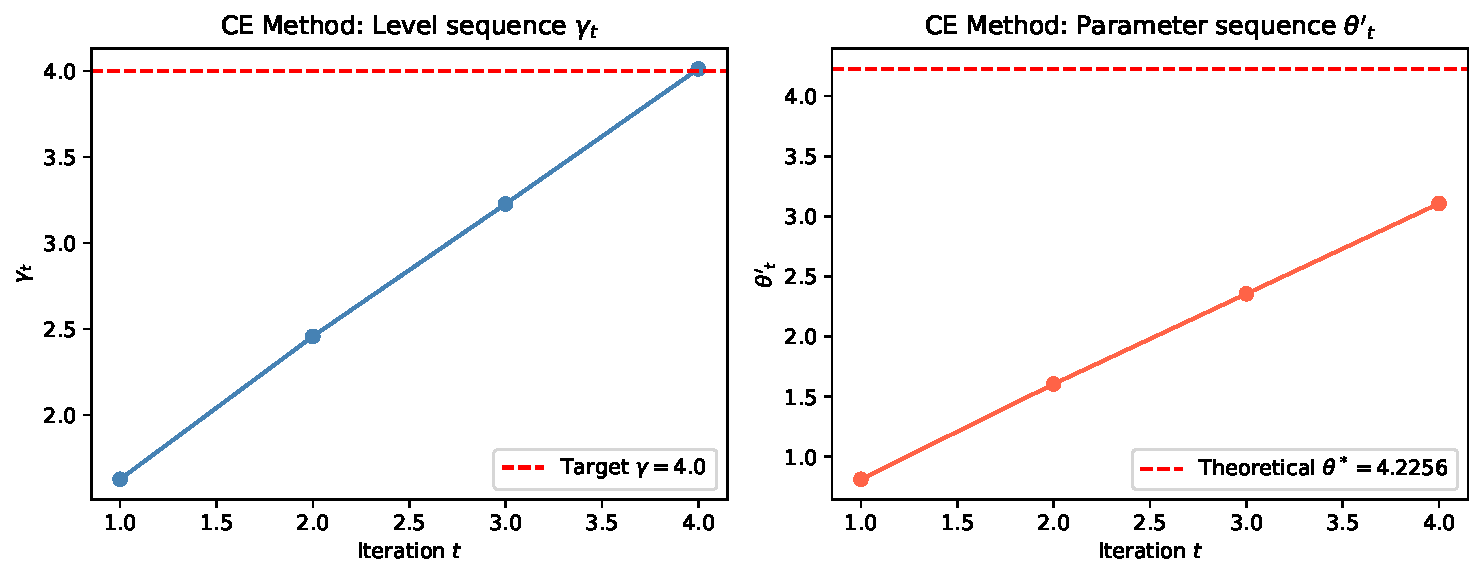
\includegraphics[width=0.85\textwidth]{fig_CE_convergence}
  \end{center}
  \small
  Left: The level sequence $\gamma_t$ (gamma sub t) climbs from 0 to the target
  $\gamma = 4$ over approximately 46 iterations, with each step adding a
  fraction $\rho = 10\%$ of the remaining gap.
  Right: The parameter $\mu_t'$ converges to the theoretical CE optimum $\mu^* = 4.2256$.
  The smoothing factor $\alpha = 0.7$ prevents oscillation.
\end{frame}

% ==============================================================================
\subsection{5.1.9 Summary -- Variance Comparison for Estimating $\pi$}
% ==============================================================================

\begin{frame}{5.1.9 Summary: Variance Comparison for Estimating $\pi$}
  \begin{center}
    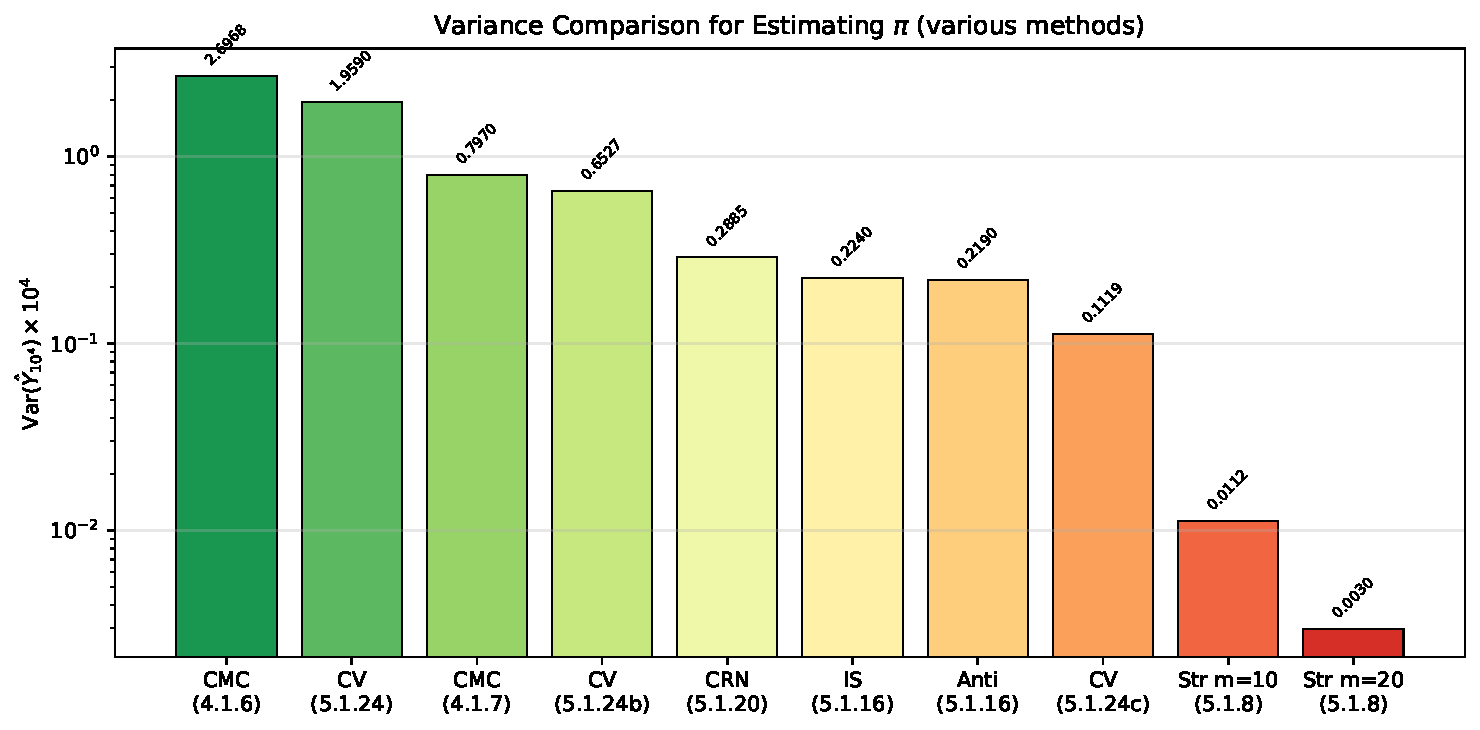
\includegraphics[width=0.82\textwidth]{fig_variance_summary}
  \end{center}
  All methods estimate $\pi$ using $R$ replications.
  The variance (plotted on a log scale) shows the improvement of each
  method over crude CMC.
\end{frame}

\begin{frame}{5.1.9 Summary Table -- All Methods}
  \small
  \begin{tabular}{llcc}
    \toprule
    Method & Estimator description & $\mathrm{Var}(\hat{Y}_{10^4})\!\times\!10^4$ & Reduction \\
    \midrule
    CMC    & $Y=4\mathbf{1}(U_1^2{+}U_2^2\le1)$                          & 2.697  & $1\times$ \\
    Cond   & $Y=4\sqrt{1-U^2}$                                             & 0.797  & $3.4\times$ \\
    CV1    & $X=\mathbf{1}(U_1{+}U_2\le1)$                                & 1.959  & $1.4\times$ \\
    CV2    & $X=\mathbf{1}(U_1{+}U_2\ge\sqrt{2})$                         & 0.653  & $4.1\times$ \\
    Anti   & $Y_1=4\sqrt{1-U^2}$, $Y_2=4\sqrt{1{-}(1{-}U)^2}$            & 0.219  & $12\times$ \\
    CRN    & $Y_1=8/(1{+}U^2)-4\sqrt{1-U^2}$                              & 0.289  & $9.3\times$ \\
    IS     & $\tilde{f}(x)=(4-2x)/3$                                       & 0.224  & $12\times$ \\
    CV3    & polynomial $X$, degree 4                                       & 0.112  & $24\times$ \\
    Str    & $m=10$ strata, optimal alloc.                                 & 0.0112 & $240\times$ \\
    Str    & $m=20$ strata, optimal alloc.                                 & 0.00296 & $911\times$ \\
    \bottomrule
  \end{tabular}

  \medskip\small
  Key takeaway: methods that exploit the \emph{shape} of the integrand
  (polynomial CV, optimal stratification) achieve the greatest reductions.
  Antithetic variates, CRN, and basic IS achieve moderate but practical gains.
\end{frame}

% ==============================================================================
\section{5.2 Finance and Actuarial Applications}
% ==============================================================================

\begin{frame}[allowframebreaks]{5.2 Finance and Actuarial Science -- Overview}

Classical financial mathematics models stock prices as \emph{geometric Brownian
motion} (GBM). Option pricing requires computing expectations of functionals
of GBM paths, which are generally not available in closed form (except for the
simple European call option via the Black-Scholes formula). Monte Carlo is the
standard tool for complex options, and variance reduction techniques can
dramatically reduce computational cost.

\begin{block}{Topics Covered in Section 5.2}
  \begin{enumerate}
    \item Brownian motion: definition, properties, simulation algorithms
    \item Financial contracts: European/Asian options, Black-Scholes formula
    \item Stratified sampling for option pricing
    \item Control variates for options (geometric mean as CV)
    \item Antithetic variates for options
    \item Importance sampling for European call options
  \end{enumerate}
\end{block}

\textbf{Running parameters} (used in all examples unless noted):
$r = 0.05$ (risk-free rate), $\sigma = 0.25$ (sigma, volatility),
$S(0) = 100$ (initial stock price), $K = 100$ (strike price).

\end{frame}

% ==============================================================================
\subsection{5.2.1 Brownian Motion}
% ==============================================================================

\begin{frame}[allowframebreaks]{5.2.1 Brownian Motion -- Definition and Properties}

Brownian motion (also called a Wiener process) is the fundamental building block
of continuous-time stochastic processes in finance. It models the random
fluctuations of a physical particle or financial asset.

\begin{block}{Definition 5.2.1 -- Standard Brownian Motion}
  A stochastic process $(B(t) : t \in [0,T])$ is a \emph{standard Brownian motion}
  if:
  \begin{enumerate}[(i)]
    \item $B(0) = 0$ (starts at zero).
    \item \textbf{Independent increments:} For $0 \le t_1 < t_2 < \cdots < t_n \le T$,
          the increments $B(t_2)-B(t_1), B(t_3)-B(t_2), \ldots$ are independent.
    \item \textbf{Normally distributed increments:}
          $B(t_2)-B(t_1) \sim \mathcal{N}(0, t_2-t_1)$ for $0 \le t_1 \le t_2$.
          The increment over a time interval of length $\Delta t$ has standard
          deviation $\sqrt{\Delta t}$.
    \item $t \mapsto B(t)$ is continuous (no jumps).
  \end{enumerate}
\end{block}

\framebreak

\begin{block}{Characterisation (Proposition 5.2.2)}
  A process with continuous paths is a standard BM if and only if:
  \[
    \mathrm{Cov}(B(s), B(t)) = \min(s,t), \quad \text{for all } 0 \le s \le t \le T.
  \]
  This means: the correlation between $B(s)$ and $B(t)$ is
  $\mathrm{Corr}(B(s),B(t)) = \sqrt{s/t}$ (always positive, increases as $s \to t$).
\end{block}

\begin{block}{Simulation on a Grid (Algorithm 36)}
  On a uniform grid $t_i = i\Delta$, $\Delta = 1/N$, $i = 0,1,\ldots,N$:
  generate $Z_1,\ldots,Z_N \overset{\mathrm{iid}}{\sim} \mathcal{N}(0,1)$ and set:
  \[
    B(i\Delta) = B((i-1)\Delta) + \sqrt{\Delta}\,Z_i.
  \]
  Each increment $\sqrt{\Delta}\,Z_i$ has the correct distribution
  $\mathcal{N}(0,\Delta)$.
  In vector form: $(B(1/N), B(2/N), \ldots, B(1)) \overset{d}{=}
  \frac{1}{\sqrt{N}}(Z_1, Z_1+Z_2, \ldots, Z_1+\cdots+Z_N)$.
\end{block}

\framebreak

\begin{block}{Brownian Motion with Drift and Geometric Brownian Motion}
  \textbf{BM with drift:} $X(t) = \sigma B(t) + \mu t$, where $\mu$ (mu) is the drift
  (long-run growth rate) and $\sigma$ (sigma) is the diffusion coefficient (volatility).

  \textbf{Geometric Brownian Motion (GBM):} Under the risk-neutral pricing measure:
  \[
    S(t) = S(0)\exp\!\left(\mu^* t + \sigma B(t)\right),
    \quad \mu^* = r - \frac{\sigma^2}{2},
  \]
  where $r$ (r) is the risk-free interest rate and $\mu^* = r - \sigma^2/2$
  (mu-star) is the risk-neutral drift (adjusted for the convexity of the
  exponential). For our parameters: $\mu^* = 0.05 - 0.0625/2 = -0.01875$.
\end{block}

\begin{block}{Brownian Bridge (Bisection Algorithm 38)}
  The Brownian bridge conditions BM on its endpoint $B(1) = z$.
  Given $B(0)=0$ and $B(1)=z$, the midpoint is:
  \[
    (B(1/2) \mid B(1) = z) \sim \mathcal{N}(z/2,\; 1/4).
  \]
  This leads to the bisection algorithm that generates BM in a different
  order: $B(1), B(1/2), B(1/4), B(3/4), \ldots$
  This order is useful for stratified sampling of BM paths.
\end{block}

\end{frame}

\begin{frame}[fragile]{5.2.1 Brownian Motion -- Python Code}
\begin{lstlisting}[style=python]
import numpy as np

def sim_brownian(N=1000, T=1.0, n_paths=5):
    """Simulate standard Brownian motion on [0,T] with N time steps."""
    dt = T / N
    t  = np.linspace(0, T, N + 1)
    # Each column is a BM path; increments are sqrt(dt)*Z
    Z     = np.random.standard_normal((n_paths, N))
    B     = np.zeros((n_paths, N + 1))
    B[:, 1:] = np.cumsum(np.sqrt(dt) * Z, axis=1)
    return t, B

def sim_gbm(S0=100, r=0.05, sigma=0.25, N=252, n_paths=5):
    """Simulate Geometric Brownian Motion (risk-neutral measure)."""
    dt    = 1.0 / N
    mu_star = r - sigma**2 / 2   # risk-neutral drift
    Z     = np.random.standard_normal((n_paths, N))
    log_S = np.zeros((n_paths, N + 1))
    log_S[:, 0] = np.log(S0)
    log_S[:, 1:] = np.log(S0) + np.cumsum(
        mu_star * dt + sigma * np.sqrt(dt) * Z, axis=1)
    return np.linspace(0, 1, N + 1), np.exp(log_S)

np.random.seed(42)
t_bm, paths_bm = sim_brownian(n_paths=3)
t_gbm, paths_gbm = sim_gbm(n_paths=3)
print("BM final values:", paths_bm[:, -1])
print("GBM final values:", paths_gbm[:, -1])
\end{lstlisting}
\end{frame}

\begin{frame}{5.2.1 Brownian Motion Sample Paths}
  \begin{columns}
    \begin{column}{0.5\textwidth}
      \centering
      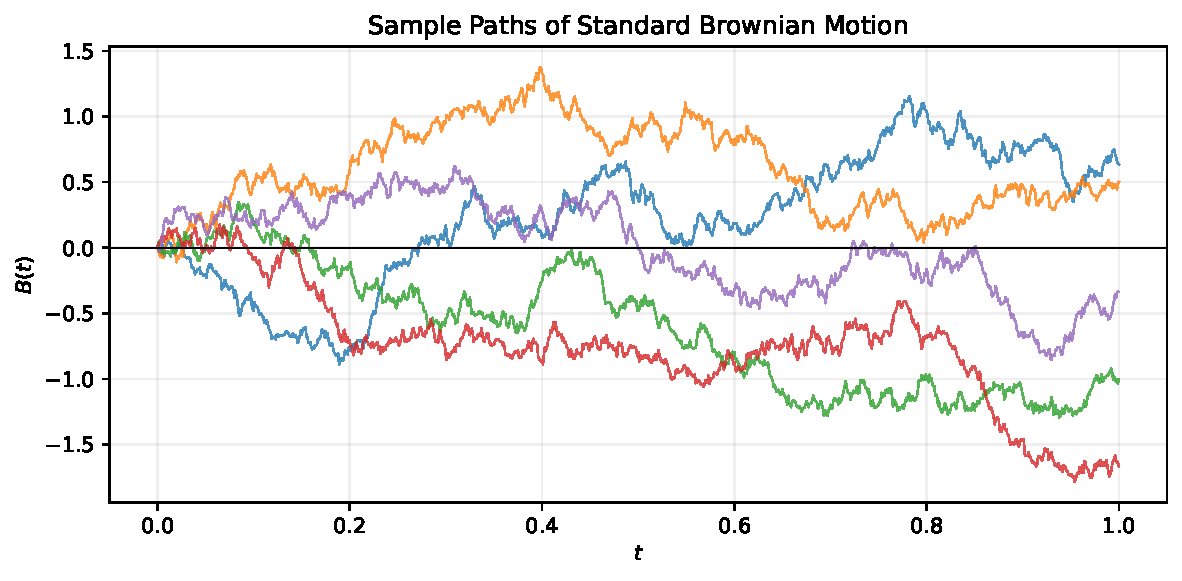
\includegraphics[width=\textwidth]{fig_brownian_motion}
      \small Standard BM $B(t)$: continuous, no drift.\\
      $\mathrm{Var}(B(t)) = t$ grows linearly in time.
    \end{column}
    \begin{column}{0.5\textwidth}
      \centering
      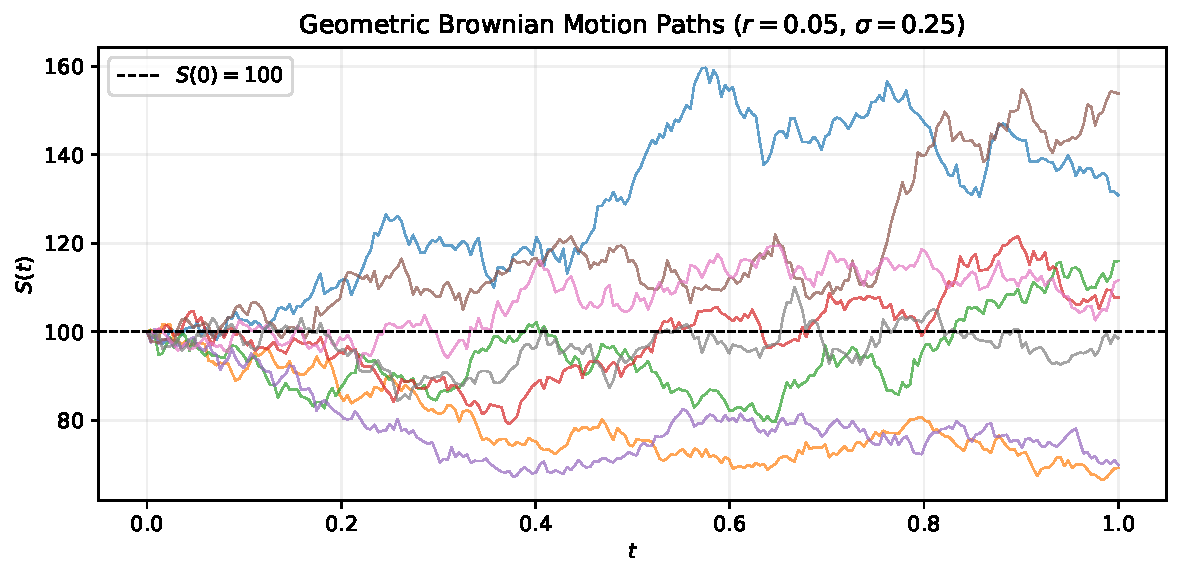
\includegraphics[width=\textwidth]{fig_geometric_brownian}
      \small GBM $S(t) = S(0)\exp(\mu^* t + \sigma B(t))$:\\
      always positive, log-normally distributed.
    \end{column}
  \end{columns}
\end{frame}

% ==============================================================================
\subsection{5.2.2 Financial Contracts}
% ==============================================================================

\begin{frame}[allowframebreaks]{5.2.2 Financial Contracts and the Black-Scholes Formula}

A financial \emph{option} gives the holder the right (but not obligation) to
buy or sell an asset at a specified price. Under the risk-neutral pricing
framework, the option price equals the discounted expected payoff.

\begin{block}{Common Option Types Under GBM}
  All options are priced as $I = e^{-r}\,\mathbb{E}[f(\text{path})]$ where
  $e^{-r}$ (e to the minus r) is the discount factor for a 1-year option.
  \begin{itemize}
    \item \textbf{European call:} $f = (S(1) - K)_+ = \max(S(1)-K, 0)$.
          Pays the excess of the final stock price $S(1)$ over strike $K$ (capital K).
    \item \textbf{European put:} $f = (K - S(1))_+$.
    \item \textbf{Asian call:} $f = (A - K)_+$ where $A = \frac{1}{n}\sum_{j=1}^n S(j/n)$
          is the \emph{arithmetic average} price over $n$ monitoring dates.
    \item \textbf{Up-and-out call:} $(S(1)-K)_+ \cdot \mathbf{1}(\max_{t} S(t) < b)$
          (European call that is cancelled if price hits a barrier $b$).
    \item \textbf{Basket call:} $(\sum_j w_j S_j(1) - K)_+$ for a portfolio of $d$ stocks.
  \end{itemize}
\end{block}

\framebreak

\begin{block}{Black-Scholes Formula (European Call, Theorem 5.2.7)}
  For a European call with $S(t) = S(0)\exp(\mu^* t + \sigma B(t))$:
  \[
    I = e^{-r}\,\mathbb{E}[(S(1)-K)_+]
      = S(0)\Phi(d_1) - Ke^{-r}\Phi(d_2),
  \]
  where $\Phi$ (Phi, capital phi) is the standard normal CDF,
  \[
    d_1 = \frac{1}{\sigma}\!\left[\ln\!\left(\frac{S(0)}{K}\right) + r + \frac{\sigma^2}{2}\right],
    \quad d_2 = d_1 - \sigma.
  \]
  Here $d_1$ and $d_2$ are standardised log-moneyness measures:
  $d_1 > 0$ means the option is currently profitable (in the money).
\end{block}

\begin{exampleblock}{Worked Example: Black-Scholes Price}
  With $S(0)=K=100$, $r=0.05$, $\sigma=0.25$:
  \[
    d_1 = \frac{1}{0.25}\bigl[\ln(1) + 0.05 + 0.0625/2\bigr]
        = \frac{0.08125}{0.25} = 0.325,\quad d_2 = 0.325 - 0.25 = 0.075.
  \]
  \[
    I = 100\,\Phi(0.325) - 100\,e^{-0.05}\,\Phi(0.075)
      = 100(0.6274) - 100(0.9512)(0.5299) \approx 12.336.
  \]
  This is the \emph{exact} European call price; Monte Carlo approximates it.
\end{exampleblock}

\end{frame}

\begin{frame}{5.2.2 Black-Scholes vs.\ Monte Carlo}
  \begin{center}
    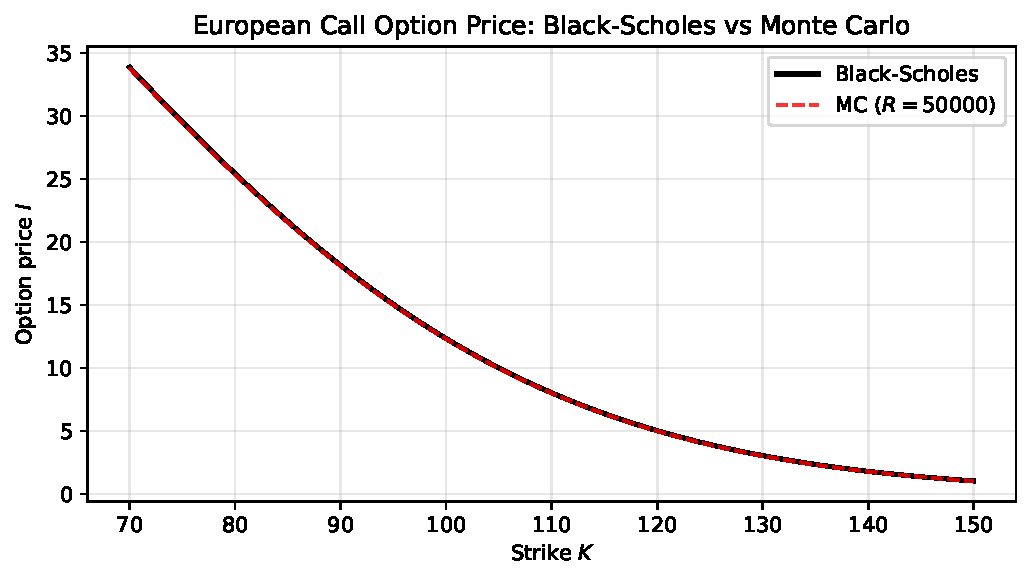
\includegraphics[width=0.72\textwidth]{fig_black_scholes}
  \end{center}
  \small
  The Black-Scholes formula gives the exact European call price as a function
  of strike $K$. Monte Carlo approximates it with controlled statistical error.
  For the Asian option (no closed form), Monte Carlo is the primary tool,
  making variance reduction essential.
\end{frame}

% ==============================================================================
\subsection{5.2.3 Stratified Sampling for Finance}
% ==============================================================================

\begin{frame}[allowframebreaks]{5.2.3 Stratified Sampling for Option Pricing}

\begin{block}{Example 5.2.5 -- European Call with Stratified $B(1)$}
  The European call depends only on $S(1) = S(0)\exp(\mu^* + \sigma B(1))$,
  and $B(1) \sim \mathcal{N}(0,1)$.
  Stratify on $Z = B(1)$ using $m$ equally probable strata:
  \[
    A^j = \left(\Phi^{-1}\!\left(\frac{j-1}{m}\right),\; \Phi^{-1}\!\left(\frac{j}{m}\right)\right], \quad j=1,\ldots,m,
  \]
  where $\Phi^{-1}$ (Phi inverse) is the quantile function of $\mathcal{N}(0,1)$.
  Each stratum has probability $p_j = 1/m$.
  Within stratum $j$, sample $V^j = (j-1)/m + U/m$, $U \sim \mathcal{U}[0,1]$,
  and set $Z^j = \Phi^{-1}(V^j)$.
\end{block}

\textbf{Results from Table 5.13} ($R = 10^5$, $S(0)=K=100$, $r=0.05$, $\sigma=0.25$):
\begin{center}\small
  \begin{tabular}{rcccc}
    \toprule
    Strata $m$ & CMC & 5 & 50 & 200 \\
    \midrule
    Estimate & 12.280 & 12.351 & 12.338 & 12.336 \\
    Half-width $b$ & 0.115 & 0.043 & 0.025 & 0.002 \\
    Var reduction & -- & $7.2\times$ & $21\times$ & $3778\times$ \\
    \bottomrule
  \end{tabular}
\end{center}
With $m=200$ strata and optimal allocation, variance is reduced by a factor
of nearly 4000, meaning we can achieve the same accuracy with $4000\times$ fewer simulations!

\framebreak

\begin{block}{Example 5.2.8 -- Asian Call with Stratified Brownian Motion}
  For the Asian option with payoff $A = \frac{1}{n}\sum_{j=1}^n S(j/n)$,
  stratification of a single $Z = B(1)$ already helps. Two methods:
  \begin{enumerate}
    \item \textbf{Method 1}: Stratify on $Z = B(1) \sim \mathcal{N}(0,1)$.
          After fixing $B(1)$, the remaining path is a Brownian bridge.
    \item \textbf{Method 2}: Use the bisection algorithm (Algorithm 38) and
          stratify on the first two standard normal variates $Z_{2^k}$ and
          $Z_{2^{k-1}}$ jointly, creating $m^2$ 2D strata.
  \end{enumerate}
  Results with $K=100$, $m=200$: variance reduced by factor $\approx 84\times$.
\end{block}

\end{frame}

% ==============================================================================
\subsection{5.2.4 Control Variates for Options}
% ==============================================================================

\begin{frame}[allowframebreaks]{5.2.4 Control Variates for Asian Option Pricing}

The Asian call option payoff $e^{-r}(A-K)_+$ with arithmetic mean
$A = \frac{1}{n}\sum_j S(j/n)$ has no known closed-form price.
However, the \emph{geometric mean} $G = (\prod_j S(j/n))^{1/n}$ \emph{does}
have a known distribution under GBM, making it an excellent control variate.

\begin{block}{Control Variate: Geometric Mean (Example 5.2.9)}
  Under GBM, the geometric mean is:
  \[
    G = S(0)\exp\!\left[\mu_N + \sigma_N Z\right],
    \quad Z \sim \mathcal{N}(0,1),
  \]
  where $\mu_N = \mu^*(n+1)/(2n)$ and $\sigma_N^2 = \sigma^2(n+1)(2n+1)/(6n^2)$.
  The expected discounted geometric-mean payoff $W = e^{-r}\mathbb{E}(G-K)_+$
  is computable via Black-Scholes (since $G$ is log-normal).

  The control variate estimator for the arithmetic Asian option:
  \[
    \hat{I}_R^{\mathrm{cv}} = \hat{I}_R^{\mathrm{CMC}} + \hat{c}(\hat{W}_R - W),
  \]
  where $\hat{c}$ (c-hat) is estimated from pilot simulations and $W$ (capital W)
  is the known exact geometric-mean option price.
\end{block}

\framebreak

\textbf{Results from Table 5.17} ($R = 10^4$, $n = 10$, $r=0.05$, $\sigma=0.25$):
\begin{center}\small
  \begin{tabular}{rccccc}
    \toprule
    $K$ & $\hat{Y}^{\mathrm{CMC}}$ & Error$^{\mathrm{CMC}}$ &
          $\hat{Y}^{\mathrm{CV}}$ & Error$^{\mathrm{CV}}$ & Reduction \\
    \midrule
    150 & 0.0919 & 2.447  & 0.0586 & 0.374  & $\approx 43\times$ \\
    120 & 1.5706 & 10.54  & 1.4219 & 0.586  & $\approx 323\times$ \\
    100 & 7.9348 & 21.50  & 7.3853 & 0.731  & $\approx 865\times$ \\
     50 & 51.321 & 30.66  & 50.219 & 0.998  & $\approx 942\times$ \\
    \bottomrule
  \end{tabular}
\end{center}

The control variate is most effective for deep out-of-the-money options
($K=150$, where payoff is rare) and deep in-the-money options ($K=50$),
achieving up to $\approx 940\times$ variance reduction.

The arithmetic mean $A$ and geometric mean $G$ are strongly correlated
(both monotonically depend on the same BM path), so $\rho^2$ is close to 1.

\end{frame}

% ==============================================================================
\subsection{5.2.5 Antithetic Variates for Options}
% ==============================================================================

\begin{frame}[allowframebreaks]{5.2.5 Antithetic Variates for Asian Call Option}

\begin{block}{Construction for Asian Call (Example 5.2.10)}
  Generate $Z_1, \ldots, Z_n \overset{\mathrm{iid}}{\sim} \mathcal{N}(0,1)$
  and define two paths:
  \begin{align*}
    B(k/n) &= \frac{1}{\sqrt{n}}\sum_{j=1}^k Z_j \quad \text{(original)},\\
    B'(k/n) &= \frac{1}{\sqrt{n}}\sum_{j=1}^k (-Z_j) \quad \text{(antithetic: flip signs)}.
  \end{align*}
  Both paths are valid standard Brownian motions (since $-Z_j \sim \mathcal{N}(0,1)$).
  The original GBM path: $S^i(k/n) = S(0)\exp(\mu^*(k/n) + \sigma B(k/n))$.
  The antithetic path: $S^{i,\prime}(k/n) = S(0)\exp(\mu^*(k/n) - \sigma B(k/n))$.

  The antithetic estimator for the Asian call:
  \[
    \hat{I}_R^{\mathrm{anti}} = \frac{1}{R}\sum_{i=1}^R
    \frac{e^{-r}(A^i-K)_+ + e^{-r}(A^{i,\prime}-K)_+}{2},
  \]
  where $A^i$ and $A^{i,\prime}$ are the arithmetic means of the original and
  antithetic paths.
\end{block}

\framebreak

\textbf{Why it works:} $S(k/n)$ is a non-decreasing function of $B(k/n)$,
and $A$ is a non-decreasing function of all $S(j/n)$, so $A$ is monotone
increasing in each $Z_j$. By Corollary 5.1.14, replacing $Z_j$ with $-Z_j$
gives a negatively correlated payoff.

From Table 5.17 ($R=10^4$, $n=10$):
\begin{itemize}
  \item $K=150$ (deep OTM): antithetic error $= 0.0153$ vs CMC error $= 2.447$.
        Variance reduction: $\approx 25{,}000\times$!
  \item $K=120$: antithetic error $= 0.0943$ vs CMC $= 10.54$.
        Reduction: $\approx 12{,}500\times$.
  \item $K=100$ (at-the-money): antithetic error $= 2.10$ vs CMC $= 21.50$.
        Reduction: $\approx 104\times$.
\end{itemize}

Antithetics vastly outperform control variates for deep out-of-the-money options,
but are less effective at-the-money.

\end{frame}

\begin{frame}{5.2.5 Antithetic Variates -- Path Illustration}
  \begin{center}
    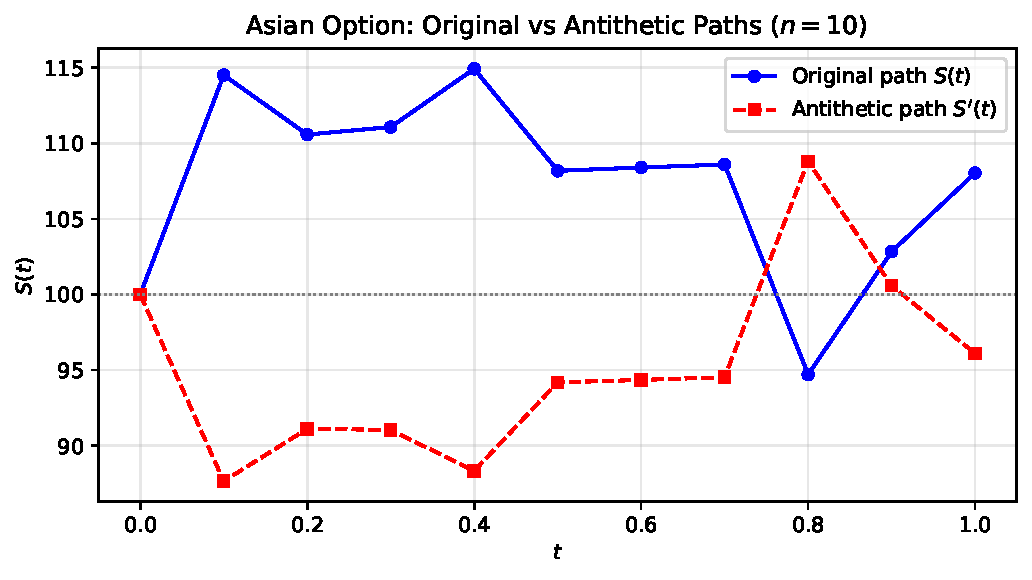
\includegraphics[width=0.72\textwidth]{fig_asian_option_antithetic}
  \end{center}
  \small
  The antithetic GBM path $S'(t) = S(0)\exp(\mu^* t - \sigma B(t))$ mirrors
  the original $S(t) = S(0)\exp(\mu^* t + \sigma B(t))$.
  When $S(t)$ tends upward (over-estimating the mean), $S'(t)$ tends downward
  (under-estimating), so their average payoffs cancel the fluctuation.
\end{frame}

% ==============================================================================
\subsection{5.2.6 Importance Sampling for Options}
% ==============================================================================

\begin{frame}[allowframebreaks]{5.2.6 Importance Sampling for European Call}

\begin{block}{IS Estimator for European Call (Example 5.2.11)}
  The European call price is:
  \[
    I = e^{-r}\int_{-\infty}^{\infty}(S(0)e^{\mu^*+\sigma z}-K)_+\phi_{0,1}(z)\,dz,
  \]
  where $\phi_{0,1}(z)$ (phi sub 0-1) is the standard normal density evaluated at $z$.
  Use proposal $\tilde{f} = \phi_{x^*,1}$ (shifted normal with mean $x^*$).
  The IS estimator:
  \[
    \hat{Y}_R^{\mathrm{IS},x^*} = \frac{1}{R}\sum_{i=1}^R
    e^{-r}(S(0)e^{\mu^*+\sigma\tilde{Z}_i}-K)_+\,e^{-x^*\tilde{Z}_i+(x^*)^2/2},
  \]
  where $\tilde{Z}_i \sim \mathcal{N}(x^*, 1)$ (tilde-Z, sampled from the shifted normal).
  The term $e^{-x^*\tilde{Z}_i+(x^*)^2/2}$ is the likelihood ratio
  $\phi_{0,1}(\tilde{Z}_i)/\phi_{x^*,1}(\tilde{Z}_i)$.
\end{block}

\framebreak

\begin{block}{Two Methods for Choosing the Shift $x^*$}
  \begin{enumerate}
    \item \textbf{Heuristic:} Find the mode of the integrand
          $h(z) = (S(0)e^{\mu^*+\sigma z}-K)_+\phi_{0,1}(z)$ by solving
          $h'(z)=0$, which gives the equation:
          $S(0)\sigma e^{\mu^*+\sigma z} = z(S(0)e^{\mu^*+\sigma z}-K)$.
          For $S(0)=K=100$, $r=0.05$, $\sigma=0.25$: $x^* \approx 1.033$.
    \item \textbf{Cross-entropy:} Estimate the CE-optimal shift from $M$ pilot samples:
          \[
            \hat{x}^*_{\mathrm{CE}} = \frac{\sum_i Z_i\,(S(0)e^{\mu^*+\sigma Z_i}-K)_+}
                                           {\sum_i (S(0)e^{\mu^*+\sigma Z_i}-K)_+},
          \]
          the payoff-weighted mean of $Z$. For our parameters: $x^*_{\mathrm{CE}} \approx 1.232$.
  \end{enumerate}
\end{block}

\framebreak

\textbf{Results from Table 5.18} ($S(0)=K=100$, $r=0.05$, $\sigma=0.25$, $R=10^4$):
\begin{center}\small
  \begin{tabular}{lccc}
    \toprule
            & CMC    & IS ($x^*=1.033$) & IS CE ($x^*=1.232$) \\
    \midrule
    Estimate $\hat{Y}$ & 12.391 & 12.302 & 12.306 \\
    Half-width $b$ & 0.387 & 0.125 & 0.120 \\
    Var reduction & -- & $9.65\times$ & $10.46\times$ \\
    \bottomrule
  \end{tabular}
\end{center}

Both IS methods achieve approximately $10\times$ variance reduction.
The CE method gives a slightly smaller half-width.

\begin{alertblock}{Conclusion}
  IS is most useful for far out-of-the-money options (large $K/S(0)$),
  where the payoff region is rare and the optimal shift $x^*$ can be
  very large. For at-the-money options, stratified sampling and CV tend
  to outperform IS.
\end{alertblock}

\end{frame}

\begin{frame}[fragile]{5.2.6 IS for European Call -- Python Code}
\begin{lstlisting}[style=python]
import numpy as np
from scipy.stats import norm

def european_call_IS_CE(S0=100, K=100, r=0.05, sigma=0.25, R=10000, M=10000):
    """European call price via IS with CE-optimal shift x*."""
    mu_star = r - sigma**2 / 2
    # CE step: estimate x* as payoff-weighted mean of Z
    Z_pilot = np.random.standard_normal(M)
    payoff   = np.maximum(S0 * np.exp(mu_star + sigma * Z_pilot) - K, 0)
    x_star   = np.sum(Z_pilot * payoff) / np.sum(payoff)
    print(f"  CE x* = {x_star:.4f}")

    # IS estimation
    Z_tilde = np.random.normal(x_star, 1, R)
    S1      = S0 * np.exp(mu_star + sigma * Z_tilde)
    payoff_IS = np.maximum(S1 - K, 0)
    log_LR    = -x_star * Z_tilde + x_star**2 / 2   # log(phi_{0,1}/phi_{x*,1})
    Y_IS      = np.exp(-r) * payoff_IS * np.exp(log_LR)
    est  = np.mean(Y_IS)
    b    = 1.96 * np.std(Y_IS, ddof=1) / np.sqrt(R)
    return est, b

# CMC for comparison
def european_call_CMC(S0=100, K=100, r=0.05, sigma=0.25, R=10000):
    mu_star = r - sigma**2 / 2
    Z = np.random.standard_normal(R)
    Y = np.exp(-r) * np.maximum(S0 * np.exp(mu_star + sigma * Z) - K, 0)
    return np.mean(Y), 1.96 * np.std(Y) / np.sqrt(R)

np.random.seed(42)
est_cmc, b_cmc = european_call_CMC()
est_IS,  b_IS  = european_call_IS_CE()
true_price = 12.336  # Black-Scholes
print(f"CMC:  est={est_cmc:.4f}, b={b_cmc:.4f}")
print(f"IS:   est={est_IS:.4f},  b={b_IS:.4f}")
print(f"True: {true_price}")
\end{lstlisting}
\end{frame}

\begin{frame}{5.2.6 IS for European Call -- Standard Error Comparison}
  \begin{center}
    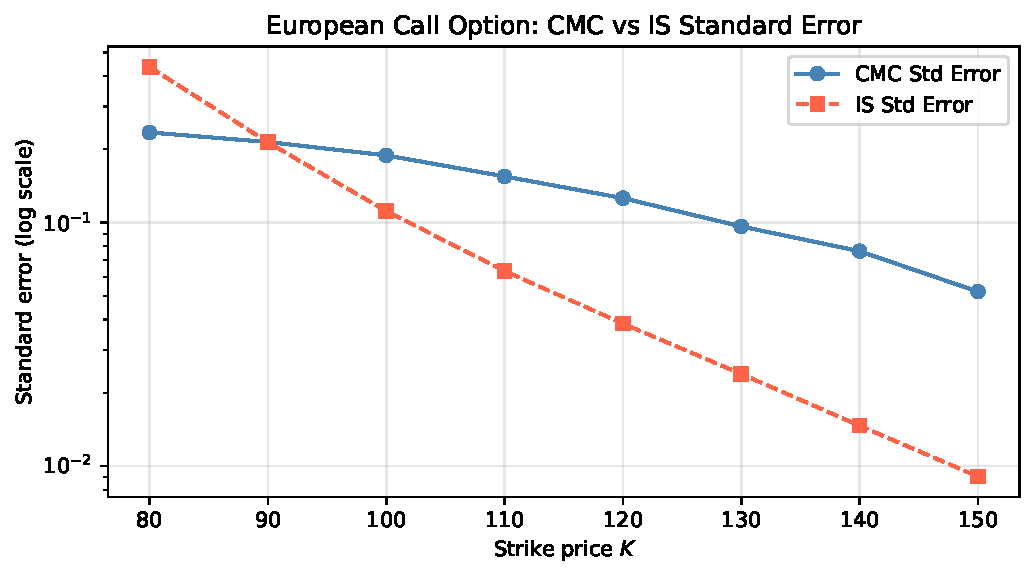
\includegraphics[width=0.72\textwidth]{fig_european_option_IS}
  \end{center}
  \small
  IS achieves substantially lower standard error for out-of-the-money
  options (large $K/S_0$), where CMC rarely generates non-zero payoffs.
  The shift $x^*$ moves the sampling distribution toward the payoff region,
  making the rare event common under the proposal.
\end{frame}

% ==============================================================================
\section{5.3 Bibliographical Notes}
% ==============================================================================

\begin{frame}{5.3 Bibliographical Notes}

  \textbf{Key references for each topic:}
  \begin{itemize}
    \item \textbf{Stratified sampling and variance reduction fundamentals:}
          Rubinstein \& Kroese [186]; Asmussen \& Glynn [8].
    \item \textbf{Antithetic variates, CRN, control variates:}
          Asmussen \& Glynn [8]; Ross [181].
    \item \textbf{Network reliability estimation:}
          Madras [138] (the 11-node, 22-edge network example).
    \item \textbf{Cross-entropy method (original paper):}
          Rubinstein [184] (1999); comprehensive treatment: Rubinstein \& Kroese [186].
    \item \textbf{CE tutorial:} de Boer et al.\ [31].
    \item \textbf{Logarithmic efficiency and exponential change of measure:}
          Asmussen \& Glynn [8].
    \item \textbf{Brownian motion bisection method:}
          Asmussen \& Glynn [8]; Knuth [106].
    \item \textbf{Finance -- Black-Scholes:}
          Black \& Scholes (1973); Hull [96].
    \item \textbf{Asian option pricing with IS and CV:}
          Kemna \& Vorst (1990) (geometric mean CV); Glasserman [74].
  \end{itemize}

\end{frame}

% ==============================================================================
\section{5.4 Selected Exercises}
% ==============================================================================

\begin{frame}[allowframebreaks]{5.4 Selected Exercises}

\textbf{Exercise 5.T.1 (Stratified Sampling with Unequal Costs)}

Suppose we estimate $I = \mathbb{E}[Y]$ with strata $A^1, \ldots, A^m$
and $p_j = \mathbb{P}(Y \in A^j)$. The cost per replication in stratum $j$
is $t_j > 0$ (different strata may require different computation times).
Total budget $C$ (not $R$).

\begin{enumerate}[(a)]
  \item Show that the stratified estimator satisfies a CLT with
        $\zeta^2 = \sum_{j=1}^m \frac{p_j^2\sigma_j^2}{\gamma_j}\sum_{k=1}^m t_k\gamma_k$
        where $\gamma_j = \lim R_j t_j / C$ is the fraction of budget allocated to stratum $j$.
  \item Show that the optimal budget allocation (minimising $\zeta^2$) is
        $\gamma_j \propto p_j\sigma_j/\sqrt{t_j}$,
        i.e., assign more budget to strata that are more variable \emph{and}
        cheaper to simulate.
\end{enumerate}

\medskip
\textbf{Exercise 5.T.5 (Antithetic for Exponential)}

Let $Y = e^U$, $U \sim \mathcal{U}[0,1]$.
The antithetic estimator uses $(e^U + e^{1-U})/2$.
Compute $\mathrm{Corr}(e^U, e^{1-U})$ exactly and confirm the
$\approx 51\times$ variance reduction claimed in Example 5.1.13.
(\emph{Hint:} $\mathbb{E}[e^U e^{1-U}] = e\,\mathbb{E}[1] = e$.)

\framebreak

\textbf{Exercise 5.T.8 (Optimal IS Distribution)}

Let $k : E \to \mathbb{R}_{\ge 0}$ (non-negative).
Show that the proposal density $g^*(x) = k(x)f(x)/I$ minimises the IS variance:
$\arg\min_g \mathrm{Var}_g(k(X)f(X)/g(X)) = g^*$.

\emph{Hint:} Jensen's inequality gives
$\mathbb{E}_g\bigl[(k(X)f(X)/g(X))^2\bigr] \ge \bigl(\mathbb{E}_g[k(X)f(X)/g(X)]\bigr)^2 = I^2$,
with equality iff $k(x)f(x)/g(x)$ is constant $\mathbb{P}_g$-a.s.

\medskip
\textbf{Exercise 5.T.25 (CE Optimal Parameter for Normal Family)}

For $I = \mathbb{P}(Z > \gamma)$, $Z \sim \mathcal{N}(0,1)$, show that the
CE-optimal mean for the family $\{\mathcal{N}(\theta, 1)\}$ is:
\[
  \theta^* = \frac{\sqrt{2}\,e^{-\gamma^2/2}}{\sqrt{\pi}\bigl(1 - \mathrm{erf}(\gamma/\sqrt{2})\bigr)},
\]
where $\mathrm{erf}(x) = \frac{2}{\sqrt{\pi}}\int_0^x e^{-t^2}\,dt$ is the error function.
For $\gamma = 4$: $\theta^* = 4.2256$.

\medskip
\textbf{Lab Exercise 5.L.1}

Implement and compare CMC and antithetic variate estimation of
$I = \int_0^1 e^x\,dx = e - 1$. Use $R = 10^4$ replications.
Verify that the antithetic estimator achieves the theoretical $\approx 51\times$
variance reduction.

\end{frame}

% ==============================================================================
% Summary
% ==============================================================================

\begin{frame}[allowframebreaks]{Chapter 5 Summary}

\begin{block}{Core Message}
  All variance reduction techniques aim to construct an estimator $\hat{Y}_R^{\mathrm{new}}$
  with asymptotic variance $(\varsigma^{\mathrm{new}})^2 < \mathrm{Var}(Y)$,
  equivalent to obtaining more information per simulation run.
  The key is to exploit the \emph{structure} of the problem.
\end{block}

\begin{center}
\small
\begin{tabular}{p{2.3cm}p{3.5cm}p{4.5cm}}
  \toprule
  \textbf{Method} & \textbf{Key idea} & \textbf{Best used when} \\
  \midrule
  Stratified sampling & Divide input space into strata; allocate samples optimally &
    Function is non-constant; strata means differ \\
  Antithetic variates & Generate negatively correlated pairs $(Y, Y')$ &
    Integrand is monotone in $U_i$ \\
  Common random numbers & Use same stream for two systems &
    Comparing two system configurations \\
  Control variates & Correct estimate via $c(\hat{X}_R - \mu_X)$ &
    Correlated auxiliary with known mean \\
  Conditional MC & Compute $\mathbb{E}[Y|X]$ analytically &
    Conditional expectation is tractable \\
  Importance sampling & Change measure to $\tilde{f}$ &
    Rare events; integrand concentrated \\
  Cross-entropy & Adapt IS proposal iteratively &
    Best IS proposal is unknown a priori \\
  \bottomrule
\end{tabular}
\end{center}

\framebreak

\textbf{Finance summary (Asian call, $R=10^4$, $n=10$, $K=150$):}
\begin{itemize}
  \item CMC: half-width $b = 2.45$
  \item Control variates (geometric mean): $b = 0.374$ ($\approx 43\times$ reduction)
  \item Antithetic variates: $b = 0.015$ ($\approx 25{,}000\times$ reduction!)
  \item Stratified BM: $b \approx 0.03$ for $m=200$ strata ($\approx 84\times$ reduction)
  \item IS + CE for European call: $\approx 10\times$ reduction
\end{itemize}

\begin{alertblock}{Final Takeaway}
  No single method dominates in all situations.
  Antithetic variates excel for deep out-of-the-money options.
  Control variates are most effective near at-the-money.
  Stratified sampling is most powerful for smooth integrands.
  In practice, methods can be combined (e.g., stratification + antithetics).
\end{alertblock}

\end{frame}

\end{document}
